\chapter{Fundamentação Teórica}
\label{cap:fundamentacao-teorica}

Neste capítulo, serão apresentadas as principais técnicas e conceitos relacionados à modelagem procedural, que servirão de alicerce para o entendimento das estratégias abordadas nesta pesquisa, a qual baseia-se na utilização de \textit{Selection Expressions}.

\section{Geração Procedural}
\label{sec:geracao_procedural}

Técnicas procedurais são segmentos de código que especificam as características de um modelo ou efeito gerado por computador. Um exemplo é a utilização de algoritmos e funções matemáticas para texturizar a superfície do mármore, ao invés da utilização de imagens escaneadas para definir o valor das cores \cite{ebert2002}.

Uma das principais vantagens da modelagem procedural é que, por meio da entrada de um conjunto regras generativas e seus respectivos parâmetros, torna-se possível criar uma grande variedade de objetos. Isto permite que a geometria real de um modelo complexo possa ser gerada apenas quando necessário \cite{smelik2014}.

\citeonline{smelik2014} argumentam que a modelagem procedural tem a capacidade de reduzir radicalmente a quantidade de esforço para criação de conteúdo digital. Contudo, boa parte dos métodos de modelagem procedural atuais ainda não oferece uma alternativa adequada em relação à modelagem manual, exigindo que os usuários manipulem regras e parâmetros não muito intuitivos, cujos efeitos na saída dificilmente podem ser previstos.

A modelagem procedural é bastante utilizada na geração de ambientes virtuais (Figura \ref{fig:virtual_world}), que são importantes em muitas aplicações, sendo algo amplamente discutido por \citeonline{smelik2010}.

\begin{figure}[h!]
	\centering
	\captionsetup{width=15cm}
	\Caption{\label{fig:virtual_world} Modelo de ambiente virtual criado com o \textit{framework SketchaWorld}: (a) ambiente natural com estrada cruzando o rio, (b) ambiente virtual final, (c) visão em perspectiva da área urbana.}	
	\UFCfig{}{
		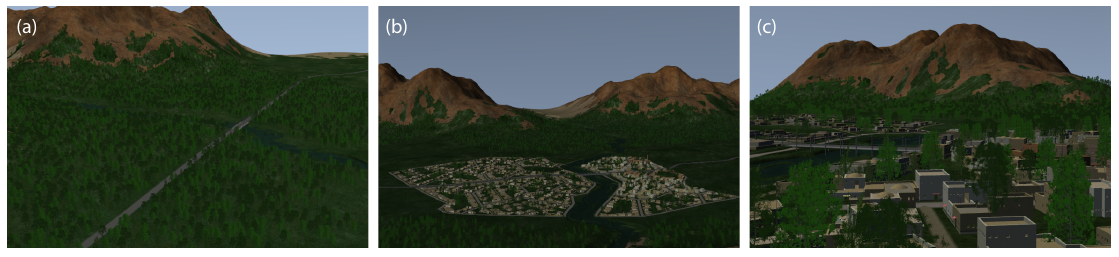
\includegraphics[width=15cm]{figuras/virtual_world.png}
	}
	{\Fonte{\cite{smelik2010}}}	
\end{figure}

Pode-se analisar a modelagem procedural de diferentes perspectivas: do poder expressivo à qualidade da produção, do tipo de interação do usuário à complexidade computacional, do grau de popularidade à área de aplicação \cite{smelik2014}, tais como geração de terrenos, vegetação, estradas, malhas fluviais, cidades e edifícios, os quais são o foco deste trabalho.

\citeonline{smelik2014} afirmam que a geração procedural de edifícios é um dos campos mais desenvolvidos da modelagem procedural, havendo ampla utilização de algum sistema de reescrita formal, como \gls{L-Systems}, \textit{split grammars} ou \textit{shape grammars}, a fim gerar um modelo de construção 3D, através de uma representação 2D.

Outros métodos alternativos, por sua vez, tentam reconstruir as gramáticas a partir de um conjunto de dados do mundo real, conforme apresentado por \citeonline{nishida2018}, com a utilização de fotografias. No exemplo mostrado na Figura \ref{fig:fachada_foto}, a) dada uma imagem e a marcação da silhueta de um edifício, b) na primeira etapa, sua abordagem estima os parâmetros da câmera e gera uma gramática de massa do edifício. Em seguida, c) a imagem da fachada é retificada e d) a gramática da fachada é gerada. Logo após, e) os elementos terminais representando as janelas são selecionados. f) Por fim, a gramática de saída é construída, e uma geometria 3D correspondente é gerada.

\begin{figure}[h!]
	\centering
	\captionsetup{width=15cm}
	\Caption{\label{fig:fachada_foto} Modelagem procedural a partir de uma imagem.}	
	\UFCfig{}{
		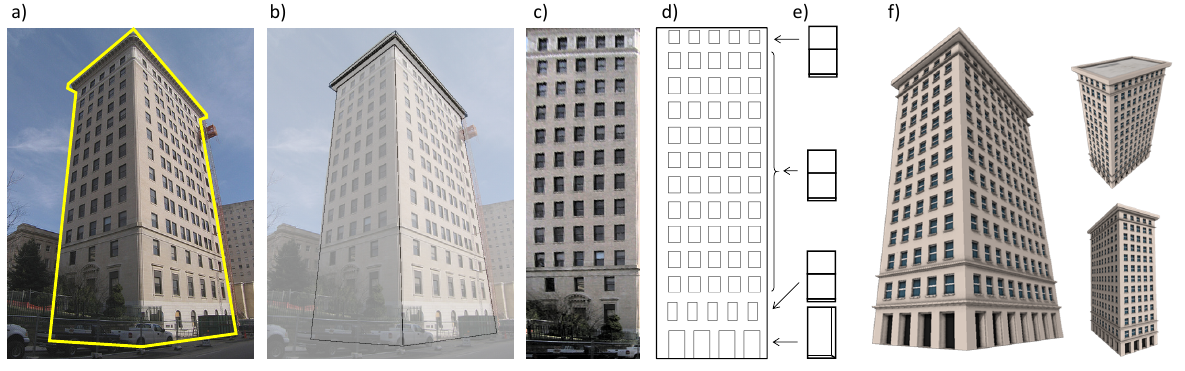
\includegraphics[width=15cm]{figuras/fachada_foto.png}
	}
	{\Fonte{\cite{nishida2018}}}	
\end{figure}

O processo de geração de edifícios por inteiro, ou seja, envolvendo fachadas e interiores, requer a utilização de métodos distintos para cada um dos casos. Na geração de fachadas, utiliza-se, geralmente, abordagens baseadas em gramáticas. Na geração de interiores, pode-se diferenciar entre a geração a partir da planta e a solução do \textit{layout} de móveis \cite{smelik2014}. O trabalho de \citeonline{leblanc2011} introduz um sistema para modelagem de edifícios completos, conforme ilustrado na Figura \ref{fig:interior}.

\begin{figure}[h!]
	\centering
	\captionsetup{width=15cm}
	\Caption{\label{fig:interior} Modelo de uma casa (à esquerda), com vista superior do primeiro andar (ao centro) e vista de dentro (à direita).}	
	\UFCfig{}{
		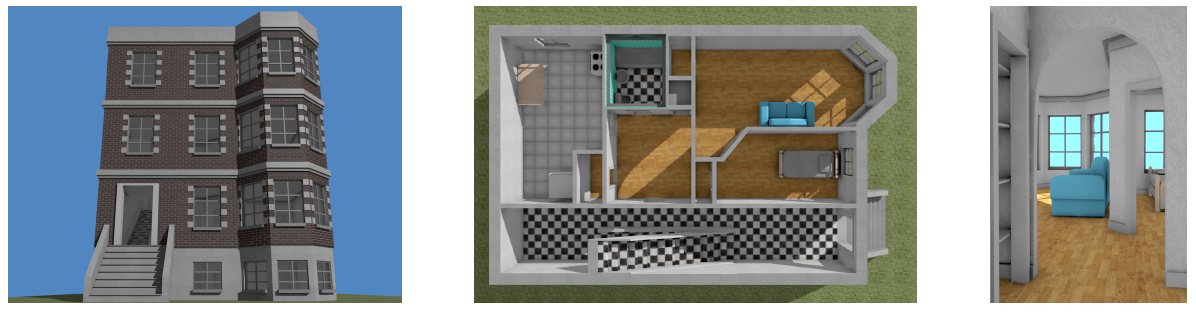
\includegraphics[width=15cm]{figuras/interior.png}
	}
	{\Fonte{\cite{leblanc2011}}}
\end{figure}

No contexto da geração procedural de edifícios, o conceito de semântica é algo primordial, pois é ela que define se a estrutura dos modelos está organizada de maneira significativa, ou seja, condizente com exemplos arquiteturais do mundo real.

Conforme argumentado por \citeonline{musse2015}, para que a geometria tridimensional de um edifício seja gerada, um conjunto mínimo de dados deve ser fornecido pelo usuário, como uma lista de arestas e vértices para definir as paredes internas de cada cômodo, ou as paredes externas do edifício, por exemplo. Na definição da parede, alguns pontos podem ser definidos para representar o centro das portas e janelas. Os quartos e suas paredes adjacentes podem receber um tipo, como cozinha, banheiro ou sala de estar. Algumas possíveis informações que podem ser definidas em uma entrada semântica são:

\begin{itemize}
    \item \textbf{Materiais:} Categorizados por tipo, como parede externa, teto e vidro, que são utilizados para restringir os tipos de materiais utilizados para cada cômodo;
    
    \item \textbf{Estilo de janelas:} Define as informações de dimensão (largura e altura), direção da abertura, profundidade da abertura, tipos de ambiente aos quais se aplica, e materiais;
    
    \item \textbf{Estilo de portas:} Semelhantes aos estilos de janelas, de modo que diferentes características possam ser consideradas, como portas com topo arredondado, portas deslizantes ou portas com painéis de vidro;
    
    \item \textbf{Estilo de telhados:} Tipos de telhados que podem ser utilizados na construção, definindo as dimensões, materiais e formas permitidas.
\end{itemize}

Portanto, uma definição semântica não é apenas uma definição de aparências, pois atribui sentido ao que está sendo criado \cite{musse2015}.

Visando construir uma linha temporal da evolução da modelagem procedural, algumas das principais técnicas precursoras são apresentadas no Apêndice \ref{ap:abordagens_precursoras}, tais como \gls{L-Systems} (Seção \ref{sec:l_systems}), \textit{Shape grammars} (Seção \ref{sec:shape_grammars}) e \textit{Split grammars} (Seção \ref{sec:split_grammar}). Então, seguindo a ordem cronológica, nas próximas seções, serão apresentadas técnicas mais recentes e pertinentes ao contexto do presente trabalho.

\section{CGA Shape}
\label{sec:cga}

A \textit{CGA Shape} foi proposta por \citeonline{muller2006} para geração procedural de modelos arquiteturais, trazendo melhorias em relação às \textit{split grammars}. Como contribuição, introduz regras de divisão com repetição, regras de redimensionamento e regras de divisão de componentes. A notação da gramática e as regras gerais para adicionar, redimensionar, transladar e rotacionar as formas são estendidas dos \gls{L-Systems}, mas voltadas para a modelagem de arquiteturas.

\subsection{Especificações}
\label{sec:cga_especificacoes}

Visando formalizar a \textit{CGA Shape}, \citeonline{muller2006} apresentam as seguintes definições e recursos:

\textbf{Forma:} Consiste em um símbolo (\textit{string}), atributos geométricos e atributos numéricos. As formas são identificadas por seus símbolos, sendo um terminal $\alpha \in \Sigma$ ou um não-terminal $\beta \in V$. As formas correspondentes são chamadas de formas terminais e formas não-terminais, respectivamente. Os atributos geométricos mais importantes são a posição $P$, três vetores ortogonais $X$, $Y$ e $Z$, que descrevem um sistema de coordenadas, bem como um vetor de tamanho $S$. Em conjunto, tais atributos definem o escopo, ou seja, uma caixa delimitadora orientada no espaço, conforme mostrado na Figura \ref{fig:cga_shape}.

\begin{figure}[h!]
	\centering
	\captionsetup{width=15cm}
	\Caption{\label{fig:cga_shape} Representação geométrica da \textit{CGA Shape}. Esquerda: definição de uma caixa delimitadora contendo uma forma primitiva. Direita: Modelo simples de uma construção utilizando três primitivas.}
	\UFCfig{}{
		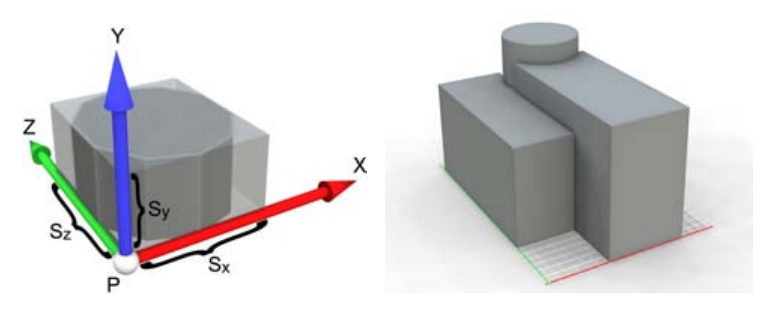
\includegraphics[width=13cm]{figuras/cga_shape.png}
	}
	{\Fonte{\cite{muller2006}}}	
\end{figure}

\textbf{Processo de produção:} Um conjunto finito de formas básicas define uma configuração. O processo de produção pode começar com uma configuração arbitrária de formas $A$, chamada de axioma, e prossegue da seguinte maneira: (1) Selecionar uma forma ativa com o símbolo $B$ no conjunto; (2) escolher uma regra de produção com $B$ no lado esquerdo para computar um sucessor para $B$, ou seja, um novo conjunto de formas $BNEW$; (3) marcar a forma $B$ como inativa, adicionando as formas $BNEW$ à configuração, e continuar com a etapa (1). O processo de produção termina quando não existirem mais não-terminais na configuração. É importante pontuar que as formas não são excluídas, mas sim marcadas como inativas, após serem substituídas. Isto permite a consulta na hierarquia de formas como um todo, e não apenas na configuração ativa.

\textbf{Notação:} As regras de produção são definidas da seguinte maneira:

\vspace{0.3cm}

\begin{description}
    \item[] \qquad \qquad $id: predecessor : cond \rightsquigarrow successor : prob$,
\end{description}

\vspace{0.3cm}

\noindent onde \textit{id} é um identificador único para a regra, $predecessor \in V$ é um símbolo que identifica uma forma que deve ser substituída por \textit{sucessor}, e \textit{cond} é uma expressão lógica que deve ser avaliada como verdadeira, antes da aplicação da regra. Uma regra, por sua vez, é selecionada com probabilidade \textit{prob}. Por exemplo, a regra:

\vspace{0.3cm}

\begin{description}
    \item[] \qquad \qquad  $1: fac(h): h > 9 \rightsquigarrow floor(h/3) floor(h/3) floor(h/3)$
\end{description}

\vspace{0.3cm}

\noindent substitui a forma de \textit{fac} por três formas \textit{floor}, se o parâmetro $h$ é maior que 9.

\textbf{Regras do escopo:} Utilizadas para modificar as formas, onde $T(t_x, t_y, t_z)$ é um vetor de translação, que é adicionado ao escopo da posição $P$; $R_x(angle)$, $R_y(angle)$ e $R_z(angle)$, gira o respectivo eixo do sistema de coordenadas; e $S(s_x, s_y, s_z)$ define o tamanho do escopo. Os símbolos $[$ e $]$ são utilizados, respectivamente, para empilhar e desempilhar o escopo atual na pilha, similar aos \gls{L-Systems}. O comando $I(objId)$ adiciona a instância de uma primitiva geométrica com identificador \textit{objId}. Objetos padrões incluem um cubo e um cilindro, contudo, qualquer modelo tridimensional pode ser utilizado. A seguinte regra define o \textit{design} do modelo de massa apresentado na Figura \ref{fig:cga_shape}:

\vspace{0.3cm}

\begin{description}
    \item[] \qquad \qquad \textit{1: A $\rightsquigarrow$ [T(0,0,6) S(8,10,18) I("cube")]}
    \item[] \qquad \qquad \, \, \, \textit{T(6,0,0) S(7,13,18) I("cube") T(0,0,16) S(8,15,8) I("cylinder")}.
\end{description}

\vspace{0.3cm}

\textbf{Regra de divisão básica}: Divide o escopo atual ao longo de um eixo. Por exemplo, considere a regra para dividir a fachada da Figura \ref{fig:cga_shape_exemplo} em quatro andares e uma saliência:

\vspace{0.3cm}

\begin{description}
    \item[] \qquad \qquad \textit{1: fac $\rightsquigarrow$ Subdiv("Y", 3.5, 0.3, 3, 3, 3)\{floor|ledge|floor|floor|floor\}}.
\end{description}

\vspace{0.3cm}

O primeiro parâmetro descreve o eixo dividido, sendo $X$, $Y$ ou $Z$, e os parâmetros restantes descrevem os tamanhos da divisão. Entre os delimitadores $\{$ e $\}$ é fornecida uma lista de formas, separadas por $|$.

\begin{figure}[h!]
	\centering
	\captionsetup{width=15cm}
	\Caption{\label{fig:cga_shape_exemplo} Exemplo de aplicação das regras da \textit{CGA Shape}. À esquerda: Um \textit{design} básico de fachada. À direita: Uma divisão simples que pode ser utilizada para os três andares superiores.}	
	\UFCfig{}{
		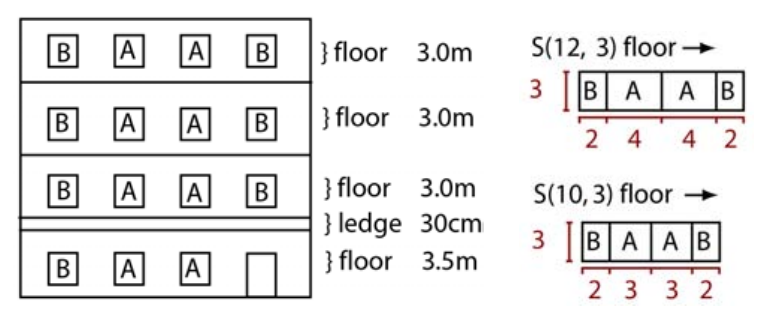
\includegraphics[width=12cm]{figuras/cga_shape_exemplo.png}
	}
	{\Fonte{\cite{muller2006}}}	
\end{figure}

\textbf{Regras de redimensionamento:} Nem todas as partes da arquitetura são redimensionadas igualmente, por isto, é possível distinguir entre valores absolutos, que não redimensionam, e valores relativos, que redimensionam. Os valores são considerados absolutos por padrão, então, para denotar valores relativos é utilizada a letra $r$, conforme a seguinte regra:

\vspace{0.3cm}

\begin{description}
    \item[] \qquad \qquad \textit{1: floor $\rightsquigarrow$ Subdiv("X", 2, 1r, 1r, 2) \{B|A|A|B\}},
\end{description}

\vspace{0.3cm}

\noindent na qual os valores relativos $r_i$ são substituídos por $r_i * (Scope.sx - \sum abs_i / \sum r_i)$, onde $Scope.sx$ representa o tamanho de $x\mbox{-}length$ do escopo atual.

\textbf{Repetição:} Permite a inclusão de um elemento específico lado a lado. Por exemplo:

\vspace{0.3cm}

\begin{description}
    \item[] \qquad \qquad \textit{1: floor $\rightsquigarrow$ Repeat("X",2) \{B\}}
\end{description}

\vspace{0.3cm}

\noindent especifica que, enquanto houver espaço, \textit{floor} será revestido com elementos do tipo $B$, ao longo do eixo x do escopo. O número de repetições é calculado a partir do valor de $repetitions = \ceil{Scope.sx/2}$.

\textbf{Divisão de componentes:} Esta nova operação permite dividir o escopo em formas de dimensões menores, conforme exemplificado no comando a seguir:

\vspace{0.3cm}

\begin{description}
    \item[] \qquad \qquad \textit{1: a $\rightsquigarrow$ Comp(type, params) \{A|B|...|Z\}},
\end{description}

\vspace{0.3cm}

\noindent onde \textit{type} identifica o tipo de divisão do componente com os parâmetros (\textit{params}) associados, se existirem. Por exemplo, \textit{Comp("faces") \{A\}} cria uma forma com o símbolo $A$ para cada face da forma tridimensional original. Da mesma maneira, \textit{Comp("edges") \{B\}} e \textit{Comp("vertices") \{C\}} são utilizados para dividir arestas e vértices, respectivamente. Para acessar apenas os componentes selecionados, são utilizados comandos como \textit{Comp("edge", 3) \{A\}}, para criar uma forma $A$ alinhada com a terceira aresta do modelo; ou \textit{Comp("side faces") \{B\}}, para acessar as faces laterais de um cubo ou cilindro poligonal. Para codificar formas de menor dimensão, são utilizados escopos cujos eixos têm tamanho diferente de zero. Para voltar à dimensões superiores, pode-se utilizar o comando $S$, com um valor não-nulo na dimensão correspondente. Por exemplo, para realizar a extrusão de uma face ao longo de sua normal e, portanto, transformá-la em uma forma volumétrica.

\subsection{Aplicações}
\label{sec:cga_exemplos}

Com objetivo de demonstrar a aplicação da \textit{CGA Shape}, \citeonline{muller2006} apresentam exemplos nos seguintes contextos:

\textbf{Prédios comerciais:} Inicialmente, é definido um conjunto de regras para gerar vários modelos com base em uma gramática estocástica. O axioma da gramática é uma forma bidimensional, representando um lote de construção. As regras, por sua vez, funcionam da seguinte maneira: na regra \ref{itm:cga_rule_1}, uma operação de extrusão é aplicada ao lote com altura definida pelo valor de $building\_height$, utilizando um comando de tamanho para produzir uma forma tridimensional. Logo após, esta forma é dividida em duas formas menores. Uma forma volumétrica, que é o maior sólido no modelo, e uma forma que, posteriormente, será dividida em duas asas laterais. Esta divisão é realizada pela regra \ref{itm:cga_rule_2}, que também gera uma lacuna entre as asas laterais. Na regra \ref{itm:cga_rule_3}, é exemplificado o uso de regras estocásticas para gerar uma variedade de modelos com diferentes configurações. Além disto, são utilizadas combinações de números aleatórios e seleção estocástica de regras, a fim de criar uma variedade de formas com diferentes alturas e larguras na asa lateral. Na regra \ref{itm:cga_rule_4}, ocorre a transição para a modelagem de fachada, permitindo que em estágios posteriores possam ser adicionadas portas e janelas, por exemplo. Um modelo gerado a partir destas quatro regras é ilustrado na Figura \ref{fig:cga_shape_models}.

\newpage

\noindent \hspace{0.5cm} PRIORITY 1:

\begin{enumerate}
    \item \label{itm:cga_rule_1} $lot \rightsquigarrow S(1r,building\_height,1r)$ \\
        \qquad \qquad \textit{Subdiv("Z",Scope.sz*rand(0.3,0.5),1r)\{ facades | sidewings \}}
    \item \label{itm:cga_rule_2} $sidewings \rightsquigarrow $ \\
        \qquad \qquad \textit{Subdiv("X",Scope.sx*rand(0.2,0.6),1r)\{ sidewing | $\epsilon$ \}} \\
        \qquad \qquad \textit{Subdiv("X",1r,Scope.sx*rand(0.2,0.6))\{ $\epsilon$ | sidewing \}}
    \item \label{itm:cga_rule_3} $sidewing$ \\
        \qquad \qquad \textit{$\rightsquigarrow$ S(1r,1r,Scope.sz*rand(0.4,1.0)) facades : 0.5} \\
        \qquad \qquad \textit{$\rightsquigarrow$ S(1r,Scope.sy*rand(0.2,0.9),Scope.sz*rand(0.4,1.0))
    facades : 0.3} \\
        \qquad \qquad$ \rightsquigarrow \epsilon : 0.2$
    \item \label{itm:cga_rule_4} \textit{facades $\rightsquigarrow$ Comp("sidefaces")\{ facade \}}
\end{enumerate}

\vspace{0.5cm}

\begin{figure}[h!]
	\centering
	\captionsetup{width=15cm}
	\Caption{\label{fig:cga_shape_models} Variações estocásticas de modelos de edifícios.}	
	\UFCfig{}{
		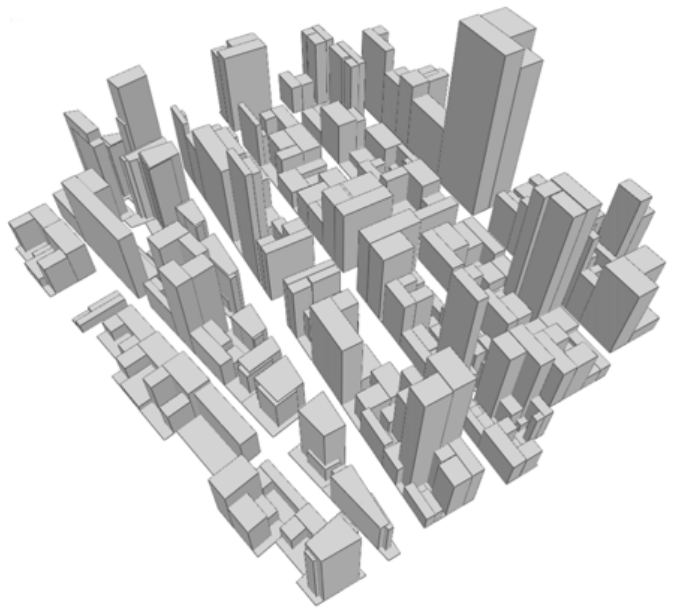
\includegraphics[width=13cm]{figuras/cga_shape_models.png}
	}
	{\Fonte{\cite{muller2006}}}	
\end{figure}

\textbf{Residências:} A gramática utilizada para gerar os ambientes da Figura  \ref{fig:cga_houses}, baseia-se na seguinte estratégia: segmentar as bordas da propriedade com uma divisão de componentes; dividir a propriedade para modelar o jardim da frente, o quintal e a construção principal; gerar uma calçada e colocar árvores em intervalos regulares ao lado da rua; e, por fim, gerar uma calçada conectada à porta da garagem, bem como uma via conectada à porta de entrada.

\begin{figure}[h!]
	\centering
	\captionsetup{width=15cm}
	\Caption{\label{fig:cga_houses} Diferentes construções em um ambiente suburbano.}	
	\UFCfig{}{
		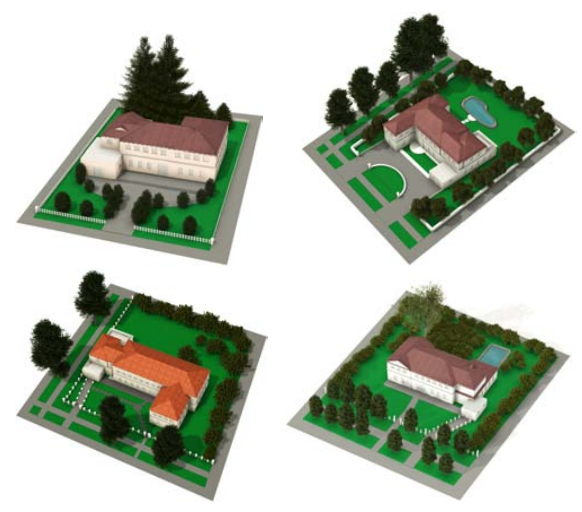
\includegraphics[width=11cm]{figuras/cga_family_houses.png}
	}
	{\Fonte{\cite{muller2006}}}	
\end{figure}

\section{CGA++}
\label{sec:cga++}

A \textit{CGA++} foi introduzida por \citeonline{schwarz2015} como sendo uma evolução natural da \textit{CGA Shape}, com o objetivo de superar algumas limitações existentes na modelagem procedural de arquiteturas, tais como:

\vspace{0.5cm}

\begin{enumerate}
    \item \label{itm:limitation_1} A coordenação do refinamento de decisões através de múltiplas formas não é diretamente suportada. Assim, qualquer decisão que afete várias formas deve ser tomada, o mais tardar, no ponto onde as linhagens destas formas divergem, para, posteriormente, ser transmitida nas regras convenientes;

    \item \label{itm:limitation_2} Normalmente, não são possíveis operações envolvendo múltiplas formas, ou seja, não são permitidas operações \textit{booleanas}, como a interseção de duas formas, nem a construção de uma forma a partir de várias outras, por exemplo;

    \item \label{itm:limitation_3} Informações contextuais, geralmente, não estão disponíveis, o que impede considerar referências de outras formas, algo necessário para determinados objetivos de modelagem, como alinhamento;

    \item \label{itm:limitation_4} O suporte para explorar múltiplas formas é inexistente. Em particular, não é possível gerar uma derivação a partir de outra derivação, e consultar ou incorporar o resultado.
\end{enumerate}

\vspace{0.5cm}

Assim, com base nestas dificuldades, \citeonline{schwarz2015} apresentam dois novos recursos com a \textit{CGA++}.

Em primeiro lugar, as formas ficam diretamente expostas na gramática, permitindo que objetos individuais sejam identificados de maneira única, bem como transmitidos e armazenados como valores. Assim, as operações podem tomar formas como argumentos, permitindo operações \textit{booleanas} em múltiplos elementos, resolvendo a limitação \ref{itm:limitation_2}. Além disto, torna-se possível acessar, percorrer e consultar a árvore de formas gerada pelo processo de derivação, o que facilita a obtenção de informações contextuais genéricas, resolvendo a limitação \ref{itm:limitation_3}. Árvores de formas temporárias podem ser criadas instantaneamente em tempo de execução, por exemplo, gerando uma nova derivação ou invocando uma função em uma árvore existente, algo que permite a busca por outras alternativas, resolvendo a limitação \ref{itm:limitation_4} \cite{schwarz2015}. 

Em segundo lugar, juntamente com o dispositivo linguístico de eventos, é fornecido um mecanismo de agrupamento dinâmico e um recurso de sincronização, permitindo a coordenação entre um grupo de formas, através da troca de informações ou do estabelecimento de uma decisão coerente sobre como proceder individualmente, resolvendo a limitação \ref{itm:limitation_1}. Além disto, os eventos podem ser utilizados para influenciar a ordem do processo de derivação, garantindo a disponibilidade de todas as formas necessárias ao realizar uma consulta contextual, resolvendo a limitação \ref{itm:limitation_3} \cite{schwarz2015}.

\subsection{Especificações}
\label{sec:especificacoes}

De acordo com \citeonline{schwarz2015}, a ideia principal para superar as limitações descritas anteriormente, na Seção \ref{sec:cga++}, é tornar as formas e a árvore de formas disponíveis na gramática. Com o processo de derivação definindo a árvore de formas, cada elemento que é gerado durante a derivação corresponde a um nó desta árvore, o que identifica ainda mais a subárvore que tem raiz neste nó. Assim, os termos \textit{forma}, \textit{nó}, e \textit{(sub)árvore} oferecem visualizações diferentes da mesma entidade. Uma vez que tal interpretação é adotada, as entidades são expostas diretamente na linguagem.

% Iniciar na próxima página
\vspace{1cm}

\citeonline{schwarz2015} argumentam que a \textit{CGA++} oferece diversas opções para fazer referência a uma forma existente. Além da consulta da árvore, as formas em um corpo de regra podem ser convenientemente acessadas por nome. Uma vez que a forma é identificada, ela pode participar livremente nas expressões; em particular, pode ser utilizada como argumento para funções e operações. Como exemplo ilustrativo, na Figura \ref{fig:cga++_exemplo_1}, a gramática (a) demonstra a operação \textit{booleana} \texttt{minus}, que modifica a forma atual subtraindo dela uma dada forma, podendo ser empregada para evitar a sobreposição de áreas na construção.

\begin{figure}[h!]
	\centering
	\captionsetup{width=15cm}
	\Caption{\label{fig:cga++_exemplo_1} Exemplo ilustrativo do uso da \textit{CGA++}: (a) gramática, (b) árvore de formas e (c) resultado.}	
	\UFCfig{}{
		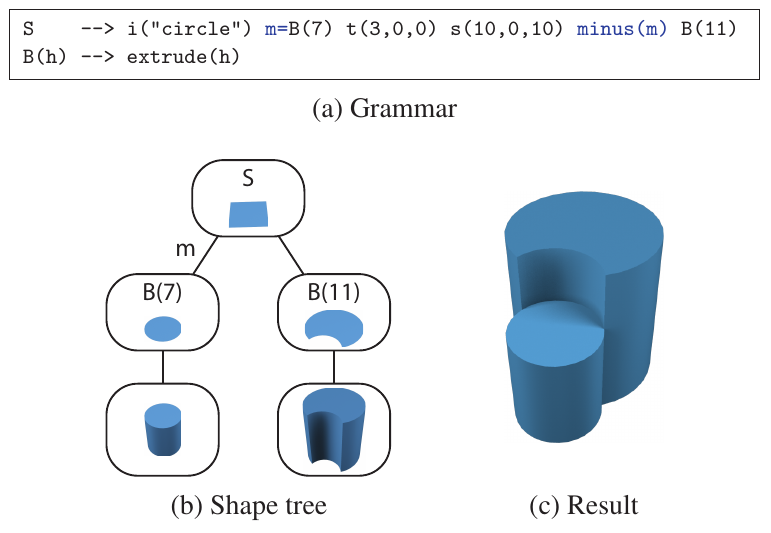
\includegraphics[width=13cm]{figuras/cga++_exemplo_1.png}
	}
	{\Fonte{\cite{schwarz2015}}}	
\end{figure}

Com objetivo de definir operações e conceitos importantes para entendimento da \textit{CGA++}, \citeonline{schwarz2015} apresentam as seguintes especificações:

\textbf{Árvore de formas:} A técnica oferece funções para navegar arbitrariamente na árvore de formas (Figura \ref{fig:cga++_arvore}). Neste contexto, dado um nó, tanto seu pai quanto sua lista de filhos podem ser consultados. Além disto, também existem funções que retornam todos os nós folha de uma dada subárvore, ou uma lista de todos os nós enumerados de acordo com uma ordem de percorrimento especificada. A ausência de um nó é denotada por \texttt{null} nas gramáticas. Para fazer referência a um nó filho rotulado, o operador de acesso associativo à esquerda \textbf{\texttt{::}} pode ser utilizado, o qual leva um nó em seu lado esquerdo e um rótulo em seu lado direito. Uma consulta na árvore de formas pode ser realizada através de atributos, permitindo abstrair a estrutura exata da árvore, o que facilita a localização de uma determinada forma com base em algum critério. Cada forma ainda pode ter um número arbitrário de atributos, que podem ser definidos e recuperados. Um atributo é identificado por um nome, e seu valor pode ser de qualquer tipo compatível com a linguagem, incluindo uma forma.

\begin{figure}[h!]
	\centering
	\captionsetup{width=15cm}
	\Caption{\label{fig:cga++_arvore} Opções de navegação na árvore. Neste caso, \texttt{a} e \texttt{b} são valores representando as formas dos nós 1 e 2, respectivamente, enquanto \texttt{X} e \texttt{Y} são rótulos.}	
	\UFCfig{}{
		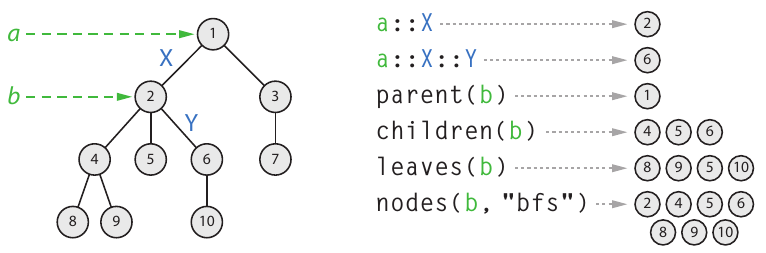
\includegraphics[width=15cm]{figuras/cga++_arvore.png}
	}
	{\Fonte{\cite{schwarz2015}}}
\end{figure}

\textbf{Novas formas:} Para gerar um novo processo de derivação dentro do atual, utiliza-se o construto \textit{<actions>(base)}, que possibilita criar uma nova árvore de (sub)formas. Assim, empregando a forma identificada por \textit{base} como forma inicial, as ações especificadas são executadas e a árvore resultante é retornada. Se o argumento \textit{base} for omitido, a forma atual é utilizada.

\textbf{Funções:} Uma nova árvore de formas é produzida por meio de várias funções internas, podendo ser derivada de uma ou mais (sub)árvores de entrada. Um conjunto destas funções se preocupa, principalmente, com a modificação de formas. Por exemplo, a função \texttt{transformScope}\textit{(source, target)} retorna uma cópia da origem, onde os escopos de todos os nós estão sujeitos à transformação, fazendo o escopo do nó raiz se tornar idêntico ao escopo de destino, ou seja, ajustando a origem no destino. Para outras operações, são fornecidas funções que tomam uma forma a ser manipulada como argumento, e retornam o resultado como uma nova forma. Por exemplo, \texttt{t}$(tree, \Delta x, \Delta y, \Delta z)$ translada os escopos de todos os nós da árvore especificada pelo deslocamento dado. Além disto, existe o grupo de funções para operações de subdivisão, cada uma retornando uma lista com todas as partes resultantes, e outro que se concentra, exclusivamente, na manipulação da estrutura da árvore.

\textbf{Formas recuperáveis:} Servem como nós indicadores que especificam como a derivação deve ser continuada em estágios futuros. Para criação de uma forma recuperável utiliza-se \texttt{?name}$(arg_0, ...)$, registrando a forma atual e os argumentos fornecidos, sendo, basicamente, um nó (forma) com atributos especiais. A função \texttt{continue}$(tree, name_0 = rule_0, ...)$ invoca a regra $rule_i$ para todas as formas recuperáveis na árvore fornecida, cujo nome corresponda a $name_i$, utilizando os argumentos associados à respectiva forma recuperável, e retorna uma árvore adequadamente refinada. Na Figura \ref{fig:formas_recuperaveis}, duas árvores de formas parciais são construídas, e a que se mostra como melhor opção é, então, completada pelo refinamento das formas recuperáveis da árvore adequada. A regra \texttt{Parcel} explora dois esquemas de desenvolvimento alternativos: primeiro, construindo parcialmente as duas árvores de formas correspondentes, depois, atribuindo às variáveis \texttt{a} e \texttt{b}, para uso subsequente. As regras \texttt{DesignA} e \texttt{DesignB}, em última análise, geram formas \texttt{Footprint} e aplicam uma operação de extrusão sobre elas, produzindo massas de construção, cujo refinamento é adiado pela emissão de uma forma recuperável \texttt{?Mass}. Empregando a função \texttt{V}, que soma os volumes das formas (folhas) de uma determinada árvore, a regra \texttt{Parcel}, então, determina a árvore com o maior volume de massa total, e continua o refinamento em suas formas recuperáveis, utilizando a regra \texttt{Mass1} ou \texttt{Mass2}, respectivamente. Por fim, a árvore de formas resultante é incorporada por meio da utilização do \texttt{include}.

\begin{figure}[h!]
	\centering
	\captionsetup{width=15cm}
	\Caption{\label{fig:formas_recuperaveis} Exemplo do uso de formas recuperáveis.}	
	\UFCfig{}{
		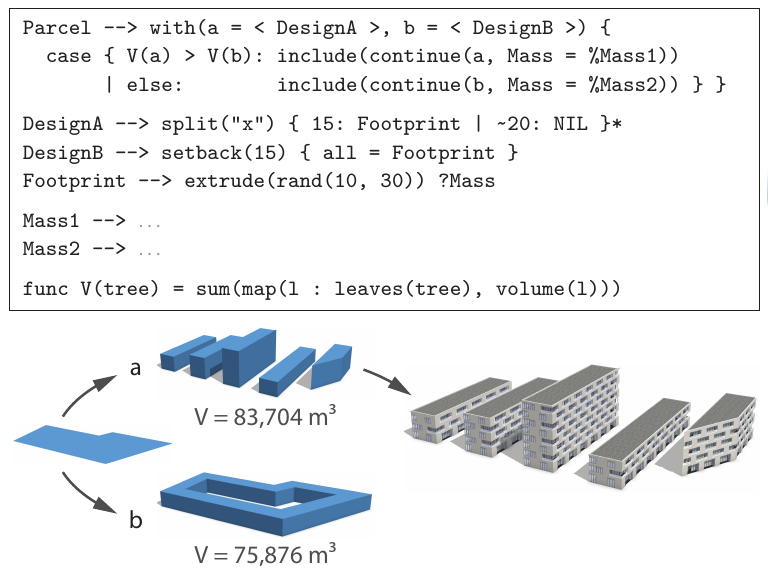
\includegraphics[width=14cm]{figuras/exemplo_formas_recuperaveis.png}
	}
	{\Fonte{\cite{schwarz2015}}}
\end{figure}

\textbf{Eventos:} Servem como pontos de sincronização, oferecendo influência na ordem em que o processo de derivação refina as formas, permitindo que vários ramos independentes da derivação troquem informações, e coordenem como proceder. São dois os principais elementos envolvidos em um evento: a operação especial \texttt{event}$(name)$ e um manipulador de eventos. A operação gera o evento especificado dentro de uma regra, que suspende a ramificação atual da derivação e a identifica como participante do evento. Uma vez que todos os ramos ativos levantaram algum evento, o manipulador de eventos é consultado. Em seguida, cada ramificação é retomada, executando a respectiva regra determinada pelo manipulador diretamente no local, o que corresponde à substituir a operação \texttt{event} pelas ações da regra. Na Figura \ref{fig:manipulador_eventos}, (1) refere-se a um evento gerado com a operação \texttt{event}, seguido de (2), que sincroniza vários ramos do processo de derivação. No \texttt{event handler} (3), recebe-se as formas atuais de todos os ramos participantes como entrada, e em (4), o manipulador do eventos retorna uma regra para cada um, especificando como proceder. 

Conforme descrito por \citeonline{schwarz2015}, o manipulador de eventos é especificado como parte da definição de um evento, sendo representado na gramática pelo seguinte construto:

\vspace{0.3cm}

\begin{description}
    \item[] \qquad \qquad $\texttt{event} \quad name(param_0 ,. . . ) \{ priority \} = handler$.
\end{description}

\vspace{0.3cm}

\citeonline{schwarz2015} afirmam que, ao fornecer parâmetros, uma família inteira de eventos pode ser definida, onde cada atribuição de parâmetro concreto constitui um evento separado, por exemplo, \texttt{e(0)} e \texttt{e(1)} são dois eventos distintos. Para cada evento é atribuído um número de prioridade, que pode depender dos valores dos parâmetros, sendo 0 se não for especificado, orientando, assim, a ordem em que múltiplos eventos concorrentes são tratados.

\begin{figure}[h!]
	\centering
	\captionsetup{width=13cm}
	\Caption{\label{fig:manipulador_eventos} Representação do manipulador de eventos.}	
	\UFCfig{}{
		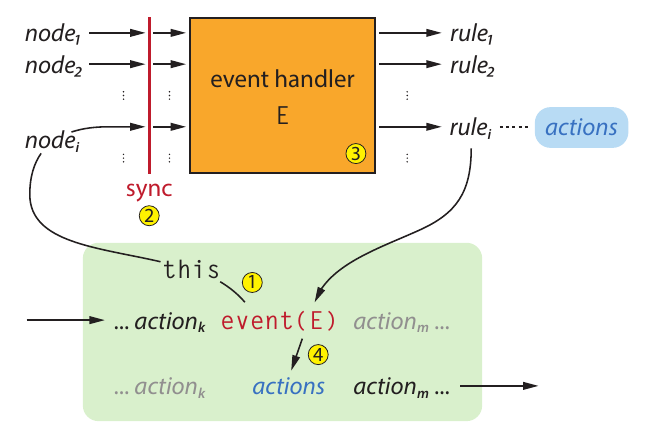
\includegraphics[width=14cm]{figuras/event_handler.png}
	}
	{\Fonte{\cite{schwarz2015}}}
\end{figure}

\subsection{Linguagem}
\label{sec:linguagem_cga++}

Os recursos da \textit{CGA++} apresentados por \citeonline{schwarz2015} ainda são complementados por outros novos componentes de linguagem, que oferecem uma notação mais simples, aumentando a expressividade, conforme mostrados a seguir:

\textbf{Objetos suportados:} Além de tipos \textit{booleanos}, números e \textit{strings}, a \textit{CGA++} oferece suporte à listas e tuplas. As listas são sequências com um número arbitrário de valores do mesmo tipo. As tuplas representam sequências com um tamanho fixo de valores, podendo ser de tipos distintos. A \textit{CGA++} também suporta funções anônimas, como o construto $[param_0, ...](body)$, que produz um novo valor de função, onde qualquer variável fora da função referenciada na expressão \textit{body} tem seu valor capturado como parte do valor da função.

\textbf{Argumentos de expressão:} Visam facilitar a expressão e fornecer uma sintaxe sucinta, sendo suportados por muitas funções integradas que processam vários itens, como os elementos de uma lista.

\textbf{Argumentos iteráveis:} Se uma função receber uma lista como um parâmetro e avaliar um argumento de expressão para cada elemento desta lista, então, um nome significativo para acessar o respectivo elemento dentro do argumento de expressão pode ser especificado como parte do argumento da lista $(name:list)$. Se omitido, o elemento fica disponível por meio de uma variável implícita.

\textbf{Operador de cadeia:} Ao aplicar, iterativamente, uma sequência de funções a um valor, o operador de cadeia \texttt{->} pode ser útil para melhorar a legibilidade, pois aplica seu lado esquerdo como primeiro argumento ao seu lado direito. Por exemplo,

\vspace{0.3cm}

\begin{description}
    \item[] \qquad \qquad $\texttt{this -> t(2, 0, 2) -> s(2, 9, 6) -> r(30, 0, 0)}$,
\end{description}

\vspace{0.3cm}

\noindent é equivalente a

\vspace{0.3cm}

\begin{description}
    \item[] \qquad \qquad $\texttt{r(s(t(this, 2, 0, 2), 2, 9, 6), 30, 0, 0)}$.
\end{description}

\vspace{0.3cm}

\textbf{Argumentos implícitos:} Em alguns casos, existe um valor bem definido $\nu \in \mathbb{N}$, no qual, geralmente, uma função é aplicada. Visando a concisão notacional, é possível, simplesmente, omitir este valor. Por exemplo, se uma função interna aparecer dentro de um corpo de regra e aceitar uma forma como primeiro argumento, a forma atual (\texttt{this}) será utilizada automaticamente se este argumento for omitido. Da mesma maneira, a lista de formas participantes (\texttt{\$nodes}) é utilizada implicitamente como primeiro argumento em uma expressão do manipulador de eventos.

\textbf{Variáveis auxiliares:} Para lidar com expressões complexas ou utilizar o resultado de uma expressão diversas vezes, variáveis auxiliares podem ajudar a trazer clareza e facilidade de formulação. Para este fim, o construto a seguir é fornecido:

\vspace{0.3cm}

\begin{description}
    \item[] \qquad \qquad $\texttt{with}(var_1 = value_1, ..., expression)$
    \item[] \qquad \qquad $\texttt{with}(var_1 = value_1, ...) \{actions\}$,
\end{description}

\vspace{0.3cm}

\noindent permitindo atribuir valores às variáveis e, posteriormente, utilizá-los em uma expressão ou dentro dos argumentos de ações.

Mais informações sobre a \textit{CGA++} foram disponibilizadas por \citeonline{schwarz2015} como material suplementar.

\subsection{Aplicações}
\label{sec:aplicacoes_cga++}

Com intuito de demonstrar os recursos de modelagem oferecidos pela \textit{CGA++}, \citeonline{schwarz2015} apresentam os seguintes exemplos, cobrindo diferentes domínios de aplicação:

\newpage

\textbf{Planejamento urbano:} Uma tarefa comum dos planejadores urbanos é projetar o chamado bloco perimetral, ou seja, um lote de blocos com edifícios em seus limites, conforme mostrado na Figura \ref{fig:cga++_planejamento_urbano}.

\begin{figure}[h!]
	\centering
	\captionsetup{width=15cm}
	\Caption{\label{fig:cga++_planejamento_urbano} Representação de bloco perimetral. Acima: estratégia de modelagem desejada e os parâmetros envolvidos. Meio: exemplos de resultados para diferentes escolhas de parâmetros. Abaixo: exemplo de um resultado de planejamento urbano no mundo real.}	
	\UFCfig{}{
		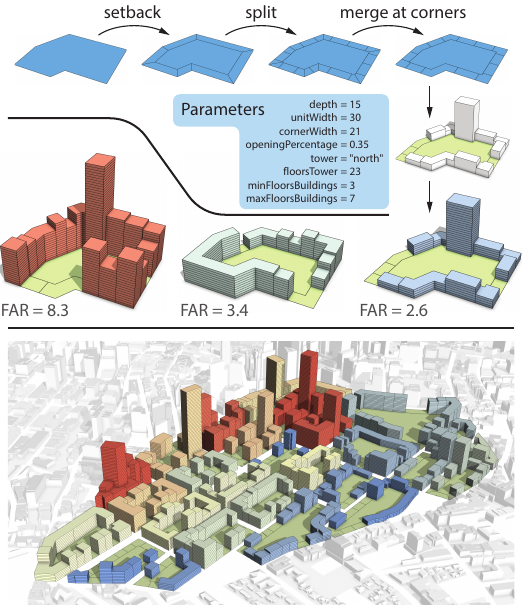
\includegraphics[width=15cm]{figuras/cga++_planejamento_urbano.png}
	}
	{\Fonte{\cite{schwarz2015}}}
\end{figure}

\clearpage
\newpage

\textbf{Edifícios:} Na Figura \ref{fig:cga++_buildings}, inspirados nos arranha-céus ecológicos de megacidades asiáticas, são apresentados modelos que consistem em, no máximo, dois blocos de torres, possuindo pisos deslocados e terraços com jardins no telhado, que são ligados por uma série de pontes suspensas.

\begin{figure}[h!]
	\centering
	\captionsetup{width=15cm}
	\Caption{\label{fig:cga++_buildings} Modelos de arranha-céus ecológicos. Acima: principais etapas da abordagem de modelagem. Abaixo: visualizações em foco do resultado do exemplo e resultados para diferentes valores para área com gramado.}	
	\UFCfig{}{
		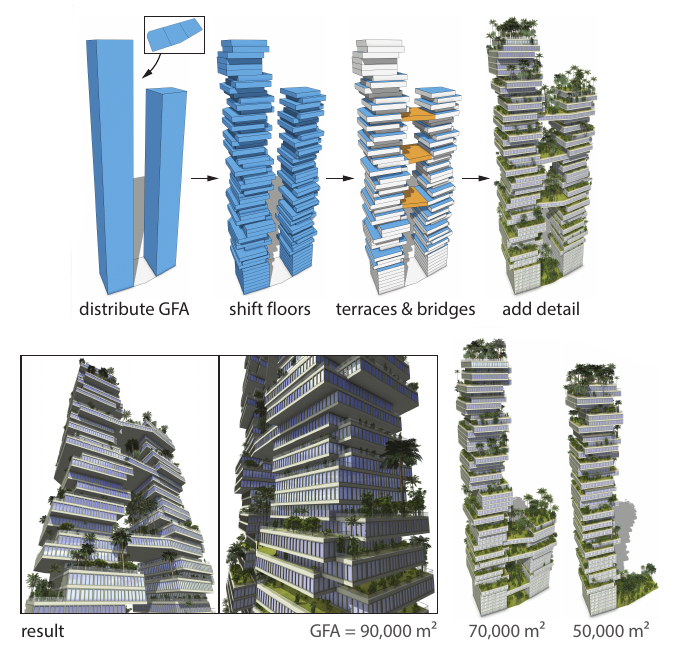
\includegraphics[width=15cm]{figuras/cga++_buildings_001.png}
	}
	{\Fonte{Adaptado de \cite{schwarz2015}}}
\end{figure}

\clearpage

\textbf{Fachadas:} Na geração de fachadas aleatórias, o alinhamento desempenha um papel fundamental, assim, as Figuras \ref{fig:cga++_fachadas} e \ref{fig:cga++_split} apresentam os recursos da \textit{CGA++} neste contexto.

\begin{figure}[h!]
	\centering
	\captionsetup{width=14cm}
	\Caption{\label{fig:cga++_fachadas} Modelos de fachadas com elementos e alinhamentos aleatórios. Acima: abordagem de solução geral, na qual as linhas de divisão são mostradas em vermelho). Abaixo: exemplo de resultados para diferentes parâmetros.}
	\UFCfig{}{
		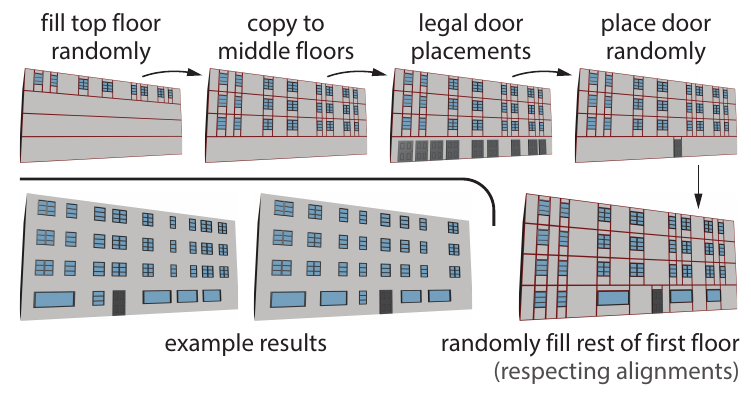
\includegraphics[width=13cm]{figuras/cga++_fachadas.png}
	}
	{\Fonte{\cite{schwarz2015}}}
\end{figure}

\begin{figure}[h!]
	\centering
	\captionsetup{width=14cm}
	\Caption{\label{fig:cga++_split} Exemplo de operação \texttt{split}, mostrando o resultado para diferentes valores de entrada, neste caso, 6 e 11.}
	\UFCfig{}{
		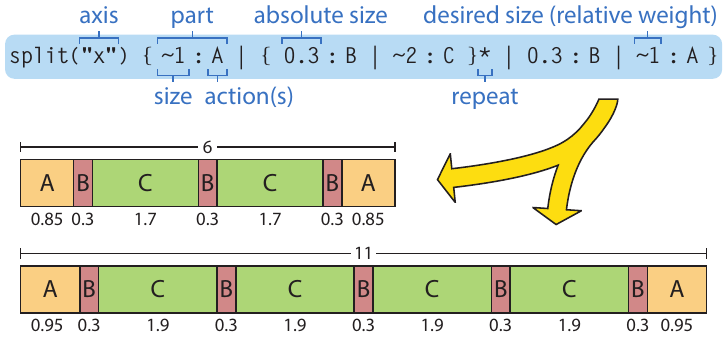
\includegraphics[width=11cm]{figuras/cga++_split.png}
	}
	{\Fonte{\cite{schwarz2015}}}
\end{figure}

\vspace{1cm}

Na próxima seção, serão apresentadas características e principais vantagens da linguagem de modelagem \textit{SELEX}, em relação às suas precursoras, previamente abordadas.

\newpage

\section{Selection Expressions}
\label{sec:selex}

A \gls{SELEX} é uma nova abordagem para geração procedural, que foi introduzida por \citeonline{wonka2018}, e tem como ideia principal selecionar formas através de \textit{selection-expressions}, substituindo a simples correspondência de \textit{strings}, utilizada em técnicas como \textit{CGA Shape} e \textit{CGA++}. 

Segundo \citeonline{wonka2018}, uma \textit{selection-expression} especifica como selecionar um subconjunto complexo de formas em uma hierarquia de formas, por exemplo, selecionar todas as janelas altas no segundo andar da fachada principal do edifício, o que permite expressar ideias de modelagem em seu contexto global. Outro recurso da \gls{SELEX} é a aplicação de restrições de alinhamento e restrições de tamanho, permitindo que descrições procedurais possam gerar variações de fachadas e construções, sem violar as restrições de alinhamento e dimensionamento que afetam o estado da arte atual. 

Para exemplificar este caso, \citeonline{wonka2018} apresentam a Figura \ref{fig:cga_problema}, que traz uma comparação entre a \textit{SELEX} e a \textit{CGA Shape}. Na coluna (a), são representados dois \textit{layouts} de fachadas. Após uma operação de redimensionamento, na coluna (b), são mostrados os resultados da \textit{CGA Shape}, e na coluna (c), os resultados da \textit{SELEX}. Pode-se perceber que algumas restrições são violadas por meio da utilização da \textit{CGA Shape}. No primeiro caso, há uma pequena diferença na largura da forma da parede no segundo andar à esquerda e à direita da fachada. Devido a esta diferença, após o redimensionamento, a regra de repetição para as janelas à esquerda e à direita produz um número diferente de repetições. No segundo caso, é mostrada uma ocorrência de desalinhamento. As janelas do segundo ao quarto andar são alinhadas no \textit{layout} de entrada. Contudo, a \textit{CGA Shape} quebra o alinhamento entre os andares três e quatro.

\begin{figure}[h!]
	\centering
	\captionsetup{width=14cm}
	\Caption{\label{fig:cga_problema} Comparação entre o \textit{layout} gerado pela \textit{CGA Shape} e \gls{SELEX}.}
	\UFCfig{}{
		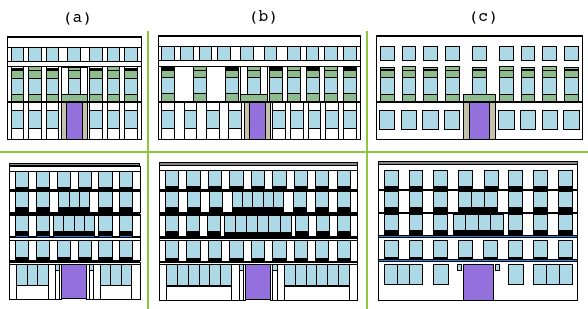
\includegraphics[width=14cm]{figuras/problema_layout.png}
	}
	{\Fonte{Adaptado de \cite{wonka2018}}}
\end{figure}

\citeonline{wonka2018} argumentam que o principal intuito de uma gramática é derivar um \textit{design} baseando-se em operações de divisão. Por exemplo, inicialmente, um modelo de massa é gerado. Logo após, as faces laterais do modelo de massa são extraídas como polígonos de fachada. Em seguida, os polígonos de fachada podem ser divididos em colunas ou pisos. Depois disto, os pisos podem ser divididos em ladrilhos e, por fim, em paredes, janelas ou portas. Desta maneira, a \gls{SELEX} visa melhorar dois problemas predominantes nesta abordagem.

Em primeiro lugar, \citeonline{wonka2018} afirmam que a \textit{CGA Shape} fornece oportunidades limitadas para coordenar os diferentes ramos da derivação. Por exemplo, uma regra pode ser invocada para um ladrilho em algum lugar de um edifício para colocar uma janela e uma varanda. Depois, esta regra precisa decidir localmente como a janela e a varanda devem ser projetadas, de modo que as decisões de \textit{design} sejam coordenadas com todos os outros elementos de um edifício. Uma vez que o alinhamento correto dos elementos é difícil de modelar, a solução proposta é a introdução de construções de linguagem que possibilitam uma melhor comunicação entre as diferentes partes de um \textit{layout}, visando utilizar uma visão global para descrever as principais decisões de \textit{design} envolvidas na modelagem. Por exemplo, ao invés das janelas decidirem localmente que tamanho, alinhamento e tipo devem ter, são escritas regras globais que descrevam onde colocar quais tipos de janelas. Assim, há uma alteração das regras no formato $label \rightarrow actions$ para regras no formato $selection\mbox{-}expression \rightarrow actions$. Enquanto trabalhos anteriores concentravam-se, principalmente, em melhorias no lado direito de uma regra, a \gls{SELEX} propõe extensões também no lado esquerdo de uma regra.

Em segundo lugar, \citeonline{wonka2018} afirmam que existem algumas desvantagens na abordagem de divisão hierárquica utilizada pela \textit{CGA Shape} e \textit{CGA++}. Por exemplo, existem diversas maneiras de ver o mesmo edifício, ou seja, olhando para uma fachada, pode-se estar interessado em expressar uma operação de modelagem em termos de pisos, em termos de colunas, ou algum subconjunto de ladrilhos. Neste contexto, a escrita da regra força um edifício a ser dividido em uma única hierarquia, o que é um problema. Assim, se o autor da regra se comprometer com uma subdivisão com base no andar, será muito difícil expressar as operações de modelagem que precisam ser coordenadas entre várias colunas e vice-versa. Por exemplo, na Figura \ref{fig:cgaVSselex}(c), a fachada é dividida em uma região à esquerda, uma coluna da porta, e uma região à direita. Em seguida, as regiões individuais são divididas em andares. Desta maneira, tal estrutura impõe uma hierarquia que tem regiões intermediárias desnecessárias que são difíceis de nomear semanticamente, e apresentam problemas para formular seleções. Para superar estas limitações, a \gls{SELEX} permite o gerenciamento de várias hierarquias simultaneamente, oferecendo suporte para múltiplas visualizações dos dados sem dividir as formas.

 Na Figura \ref{fig:cgaVSselex}, \citeonline{wonka2018} ilustram os problemas com a abordagem anterior e as vantagens do uso da \gls{SELEX}: 
 
 \begin{description}
     \item[] \; (a) Fachada vazia;
     
     \item[] \; (b) Grades são utilizadas para permitir diferentes visualizações de \textit{design}, como linhas, colunas, sub grades ou células individuais da grade;
     
     \item[] \; (c) Problemas de divisão das abordagens atuais, as quais não permitem a fusão de células. Desta maneira, ao se realizar divisões para estabelecer regiões de múltiplas células, sequências complexas e difíceis divisões verticais e horizontais alternadas são necessárias, o que é difícil de gerenciar;
     
     \item[] \; (d) A \gls{SELEX} permite selecionar, arbitrariamente, sub-grades retangulares de uma grade, e posicionar elementos em relação a elas, permitindo a modelagem de uma forma natural e semanticamente significativa;
     
     \item[] \; (e) Na geração de fachadas de edifícios, para simplificar o alinhamento, os elementos são organizados de acordo com uma grade. Contudo, elementos únicos podem abranger várias células da grade ou serem colocados entre as células da grade. Em particular, pode-se incorporar elementos que abrangem duas células, cada uma delas contendo um outro elemento, como os ornamentos amarelos e azuis no último andar. Para isto, a \gls{SELEX} fornece suporte à seleções sobrepostas, onde pode ser necessário a seleção de uma única célula para colocar cada janela, e uma seleção de célula dupla para colocar ornamentos, por exemplo.
 \end{description}
 

\begin{figure}[h!]
	\centering
	\captionsetup{width=15cm}
	\Caption{\label{fig:cgaVSselex} Ilustração dos paradigmas de modelagem \gls{SELEX} e \textit{CGA Shape}.}
	\UFCfig{}{
		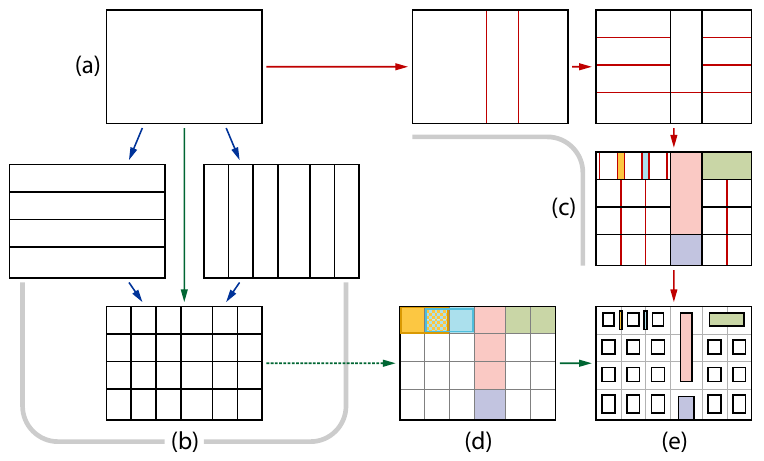
\includegraphics[width=14cm]{figuras/cgaVSselex.png}
	}
	{\Fonte{\cite{wonka2018}}}	
\end{figure}

\subsection{Definições de forma}
\label{sec:selex_definicao_formas}

\citeonline{wonka2018} argumentam que a maneira de organizar o conjuntos de formas produzidas pela linguagem é uma importante decisão de \textit{design}. Neste contexto, uma escolha é simplesmente operar em um conjunto de formas sem qualquer hierarquia, conforme mostrado na Figura \ref{fig:shapes_selex}(e). Outra abordagem clássica é organizar as formas em uma árvore, porém, isto requer o comprometimento com uma hierarquia específica. Ou seja, para fachadas, várias hierarquias (ou árvores) podem existir a qualquer momento, e as operações de modelagem são normalmente expressas em diferentes hierarquias. Por exemplo, em alguns casos, as janelas devem ser selecionadas com base nos pisos (linhas) e, outras vezes, com base nas colunas da fachada, conforme mostrado nas Figuras \ref{fig:shapes_selex}(b) e \ref{fig:shapes_selex}(c), respectivamente. Uma outra possibilidade é criar e manter explicitamente várias hierarquias em paralelo, conforme mostrado na Figura \ref{fig:shapes_selex}(d). No entanto, isto pode levar a problemas de consistência, uma vez que existe um grande número de maneiras intermediárias possíveis para agrupar outras formas.

Para solucionar este desafio \citeonline{wonka2018} utilizam grades como formas virtuais, as quais permitem o gerenciamento de qualquer sub-região como forma auxiliar, sem a necessidade de gerar a sub-região explicitamente, conforme ilustrado na Figura \ref{fig:shapes_selex}(f). Existem, assim, dois tipos de formas diferentes: formas virtuais e formas de construção. As formas virtuais possuem várias linhas e colunas, consistindo em diversas células, as quais podem ser aplicadas em formas de construção 2D, com objetivo exclusivo de orientar o posicionamento de outras formas de construção, mas não de subdividi-las. Para uma forma de construção, podem existir diversas formas virtuais, permitindo a modelagem de \textit{layouts} complexos.

Conforme apresentado por \citeonline{wonka2018}, formas virtuais podem ser utilizadas nos seguintes casos:

\begin{itemize}
    \item Alocar uma posição a partir da seleção de uma célula da grade, na qual determinada forma pode ser adicionada;
    
    \item Facilitar a seleção das formas de construção que estão contidas dentro delas, por exemplo, para selecionar formas na mesma linha ou coluna;
    
    \item Definir o comportamento de redimensionamento, uma vez que a especificação da grade inclui informações sobre o espaçamento de linhas e colunas, e a forma como as linhas e colunas se repetem, enquanto houver espaço disponível.
\end{itemize}

\begin{figure}[h!]
	\centering
	\captionsetup{width=15cm}
	\Caption{\label{fig:shapes_selex} As ilustrações (b), (c), (d), (e) e (f), representam diferentes perspectivas da árvore de formas em relação ao \textit{design} da fachada (a).}
	\UFCfig{}{
		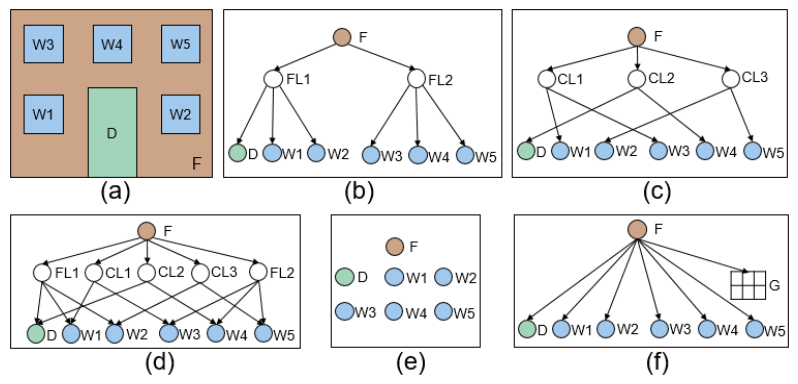
\includegraphics[width=15cm]{figuras/shapes_selex.png}
	}
	{\Fonte{\cite{wonka2018}}}	
\end{figure}

De acordo com \citeonline{wonka2018}, a \gls{SELEX} utiliza um conjunto de atributos integrados para cada forma. \textit{Label} é o nome da forma, por exemplo, \textit{"window"}. O \textit{Type} indica se a forma é uma forma virtual (\textit{"virtual"}) ou uma forma de construção (\textit{"construction"}). \textit{Dim} é uma variável binária que indica uma forma 2D ou 3D. O escopo descreve uma caixa orientada no espaço 3D, utilizando variáveis que descrevem um quadro de coordenadas $(xaxis, yaxis, zaxis)$, uma posição em $R^3$ (denotada por $xpos$, $ypos$, $zpos$), e informações de tamanho \textit{(xsize, ysize, zsize)}.

\citeonline{wonka2018} afirmam que a linguagem da \gls{SELEX} desenvolve uma hierarquia de formas e as armazena em uma árvore, por meio da utilização de certas funções. Cada forma pode ter apenas um pai, e apenas formas de construção podem ter filhos. O nó raiz é uma forma com o rótulo \textit{"root"}. As formas 2D são utilizadas para criar subdivisões em outras formas 2D, por exemplo, fachadas ou janelas. As formas 3D são utilizadas para modelar elementos que são gerados através de operações de extrusão da fachada ou estruturas suspensas, como uma varanda ou um ornamento na janela, por exemplo. Na hierarquia de formas da \gls{SELEX}, as formas têm filhos que são formas anexadas ou formas contidas. Uma forma anexada é uma forma 3D vinculada a uma forma 2D. Em algumas situações, a forma anexada tem uma face contida na forma 2D, às vezes, as formas não se tocam. Por exemplo, a forma 3D de uma varanda pode ser anexada a uma forma 2D, que descreve a posição da janela dentro de uma fachada. Uma forma contida é uma forma 2D presente dentro de sua forma 2D pai, ou uma face lateral de uma forma 3D pai. Uma forma conectada é uma forma 2D que compartilha uma aresta com outra forma 2D. Topologicamente, uma forma conectada é considerada uma vizinha no contexto de \textit{selection-expressions}. A Figura \ref{fig:shapes3D_selex} ilustra o conceito de forma contida, anexada e conectada.

\begin{figure}[h!]
	\centering
	\captionsetup{width=15cm}
	\Caption{\label{fig:shapes3D_selex} Para a forma atual (\textit{leftWall}), é demonstrada uma forma contida (\textit{win}), uma forma anexada (\textit{balcony}) e uma forma conectada (\textit{cornerWall}).}
	\UFCfig{}{
		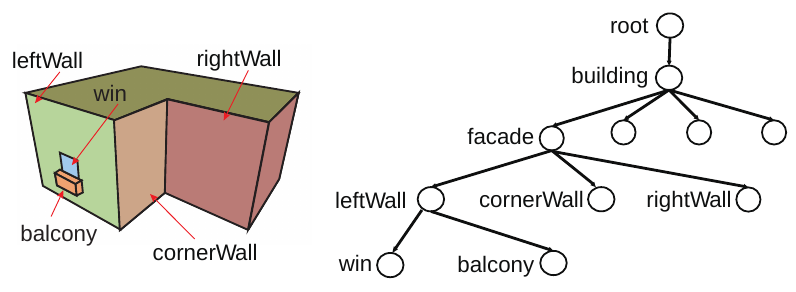
\includegraphics[width=15cm]{figuras/shapes3D_selex.png}
	}
	{\Fonte{\cite{wonka2018}}}	
\end{figure}

\subsection{Introdução à linguagem}
\label{sec:introducao_selex}

\citeonline{wonka2018} explicam que a linguagem de modelagem procedural \gls{SELEX} executa um comando por vez, podendo ser uma regra ou uma atribuição de variável. Uma regra tem o seguinte formato:

\vspace{0.3cm}

\begin{description}
    \item[] \qquad \qquad $selection\mbox{-}expression \rightarrow actions$,
\end{description}

\vspace{0.3cm}

\noindent na qual a \textit{selection-expression} seleciona uma lista de formas da árvore de formas, e as \textit{actions} são comandos a serem executados. Por exemplo, na Figura \ref{fig:code_selex}, os comandos de C2 a C11 são regras. Uma atribuição tem o formato:

\vspace{0.3cm}

\begin{description}
    \item[] \qquad \qquad $identifier = expression$,
\end{description}

\vspace{0.3cm}

\noindent na qual o \textit{identifier} denota uma variável e a \textit{expression} representa um valor. Os comandos rotulados como $C1$, na Figura \ref{fig:code_selex}, são atribuições de variáveis. Uma lista é uma lista de outros tipos de objetos, mas também há suporte para listas de listas. Um par consiste em dois objetos, no qual o primeiro objeto deve ser comparável, podendo ser um número, uma \textit{string} ou um valor \textit{booleano}, e o segundo objeto pode ser de qualquer tipo.

\begin{figure}[h!]
	\centering
	\captionsetup{width=15cm}
	\Caption{\label{fig:code_selex} Instruções \gls{SELEX} para gerar a fachada da Figura \ref{fig:cgaVSselex}(e).}
	\UFCfig{}{
		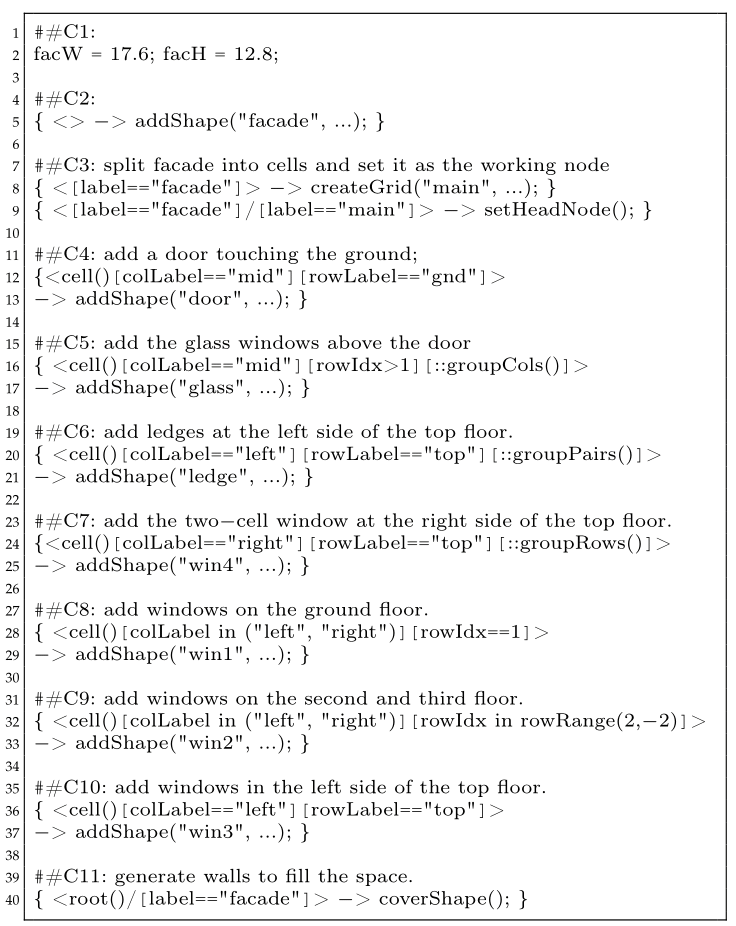
\includegraphics[width=15cm]{figuras/code_selex.png}
	}
	{\Fonte{\cite{wonka2018}}}	
\end{figure}

\subsection{Modelagem procedural baseada em seleção}
\label{sec:modelagem_selecao}

Segundo \citeonline{wonka2018}, o recurso mais importante da \gls{SELEX} são as \textit{selection-expressions}, que permitem selecionar os elementos de uma árvore de formas através de seletores intercalados com o operador $/$. Cada seletor recebe uma lista de formas como entrada e retorna uma lista de formas. A entrada implícita para o primeiro seletor é uma lista contendo o nó raiz da árvore de formas. O operador $/$ obtém uma lista de formas como entrada e executa os comandos definidos. 

\citeonline{wonka2018} argumentam que seletores são agrupados em sequências de seletores especializados, podendo ser de três tipos diferentes: seletor de topologia, como \textit{child}, \textit{descendant} e \textit{parent}; seletor de atributo, como \textit{[label=="window"]}; e seletor de grupo, como $[::groupRows()]$. Os seletores precisam ocorrer na ordem em que foram fornecidos, ou seja, não podem ser misturados em uma sequência arbitrária. 

Na definição de \citeonline{wonka2018}, uma \textit{selection-expression} possui a seguinte configuração:

\vspace{0.3cm}

\begin{description}
    \item[] \qquad \qquad \textit{<[topoS][attrS | groupS]$^*$/[topoS][attrS | groupS]$^*$/... >},
\end{description}

\vspace{0.3cm}

\noindent onde, dentro de cada sequência de seletor, há de zero a um seletores de topologia (\textit{topoS}), zero a muitos seletores de atributo (\textit{attrS}), e zero a muitos seletores de grupo (\textit{groupS}). Uma \textit{selection-expression} vazia retorna a entrada. Quando uma forma que não existe é especificada, a seleção correspondente retornará uma forma vazia e a regra não será executada. Um exemplo é mostrado na Figura \ref{fig:graph_selex}, por meio de um grafo abstrato, no qual os nós selecionados pela \textit{selection-expression} 

\vspace{0.3cm}

\begin{description}
    \item[] \qquad \qquad \textit{<[label="A"]/[label="C"][h $\geq$ 2]>}
\end{description}

\vspace{0.3cm}

\noindent são destacados em verde. No processo, a \textit{selection-expression} seleciona os filhos rotulados como "$A$" \, do nó raiz, então, para os dois nós rotulados como "$A$", todos os seus filhos rotulados como "$C$", \, com um valor de atributo $h \geq 2$, são selecionados.

\begin{figure}[h!]
	\centering
	\captionsetup{width=15cm}
	\Caption{\label{fig:graph_selex} Grafo abstrato da seleção de nós.}
	\UFCfig{}{
		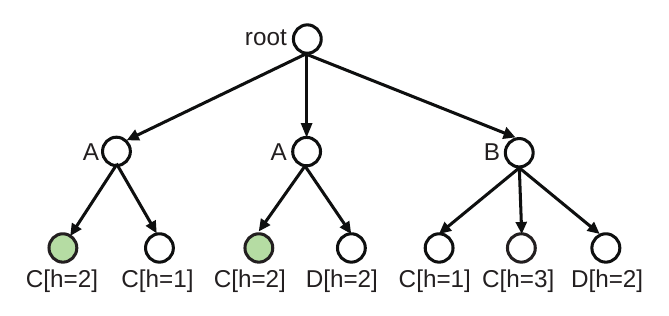
\includegraphics[width=13cm]{figuras/graph_selex.png}
	}
	{\Fonte{\cite{wonka2018}}}	
\end{figure}

Por se tratar de um importante recurso da \gls{SELEX}, \citeonline{wonka2018} apresentam algumas especificações mais detalhadas sobre os diferentes tipos de seletores:

\textbf{Seletor de topologia:} Recebe uma lista contendo uma única forma como entrada, e produz uma lista de formas com a relação de topologia especificada para a forma de entrada. Um seletor de topologia tem a forma $[topology\mbox{-}function()]$, e pode utilizar uma das seguintes funções: $child()$, $descendant()$, $parent()$, $root()$, $neighbor()$ e $contained()$.

\textbf{Seletor de atributo:} Recebe uma lista de formas e retorna uma lista de formas cujos atributos satisfazem algumas condições. Em sua estrutura básica, um seletor de atributo tem a configuração $[attribute\mbox{-}name \;\; comparison \:\; value]$. Os operadores relacionais são especificados como em outras linguagens de programação, por exemplo, $==$, $<=$, $>=$, $!=$ e $in$. Os exemplos são \textit{[label=="facade"]} e \textit{[label \, in \, ("window\_arch", "window\_rect")]}. Alternativamente, em sua estrutura mais geral, um seletor de atributo é uma expressão \textit{booleana}. Alguns outros exemplos são $[isEmpty()]$, $[numCols()>4]$ e $[toShapeX(0.5)>2]$. A função $toShapeX(0.5)$ dimensiona o valor de entrada $0.5$ pelo \textit{xsize} de uma forma. Uma função importante é a $pattern(regex, pat)$, que verifica se o padrão de caracteres de \textit{regex}, na posição do índice de uma forma, corresponde à \textit{pat}. Por exemplo, \textit{pattern("(AB)$^*$", "A")} testa se uma forma de entrada está em uma posição de índice ímpar, e \textit{pattern("A(B)$^*$A", "A")} testa se uma forma de entrada está na primeira ou na última posição de uma lista de entrada. As funções $isEven()$ e $isOdd()$ são casos especiais do comando $pattern(regex, pat)$, que verificam se uma forma tem um índice par ou ímpar em uma lista de formas selecionadas. Os atributos \textit{rowIdx} e \textit{colIdx} são utilizados como a posição topológica de uma célula em relação à região abrangida pelas formas virtuais de entrada. Por exemplo, $rowIdx==1 \, \&\& \, colIdx==1$ especifica a célula superior esquerda de uma grade. 

\textbf{Seletor de grupo:} Recebe uma lista de formas como entrada e aplica operações de agrupamento para retornar uma lista de formas combinadas. Um seletor de grupo opera apenas em formas virtuais e reagrupa sub-regiões, por exemplo, combinando células de uma forma virtual para representação de pisos. Os seletores de grupo são implementados utilizando funções de agrupamento, resultando em seletores na seguinte configuração: $[::grouping\mbox{-}function()]$. Algumas funções que operam juntamente com seletores de grupo são:

\begin{itemize}
    \item $groupRows()$ e $groupCols()$: mesclam formas virtuais adjacentes, ou seja, \textit{cells}, com o mesmo índice de linha ou coluna, respectivamente;
    
    \item $groupRegions()$: mescla todas as formas virtuais adjacentes que formam uma ou várias regiões retangulares;
    
    \item $groupEach(n)$: mescla todas as $n$ formas virtuais adjacentes.
    
    \item $groupPair()$: gera todos os pares possíveis de duas formas subsequentes. Por exemplo, dado "$ABCD$", ele retornará "$AB$", "$BC$" \, e "$CD$";
    
    \item $cells()$: decompõe uma forma virtual como uma lista de formas virtuais com uma célula.
\end{itemize}

\vspace{0.3cm}

Nas Figuras \ref{fig:seletores} e \ref{fig:agrupamento}, respectivamente, \citeonline{wonka2018} ilustram a utilização de alguns seletores e funções de agrupamento:

\vspace{0.3cm}

\begin{description}
    \item[] \; (a) Uma grade é utilizada para demonstrar múltiplas seleções;
    \item[] \; (b) \textit{<descendant()[label=="facade"]/[label=="mainGrid"]/[type=="cell"]} \\
    \qquad \qquad \qquad \textit{[rowIdx in (1,2)][colIdx==3]>};
    \item[] \; (c) \textit{<descendant()[label=="facade"]/[label=="mainGrid"]/[type=="cell"]} \\
    \qquad \qquad \qquad \textit{[rowIdx in (3,4)][colIdx in (1,2,4,5)][::groupRegions()]>};
    \item[] \; (d) \textit{<descendant()[label=="facade"]/[label=="mainGrid"]/[type=="cell"]} \\
    \qquad \qquad \qquad \textit{[rowIdx in (1,2)][colIdx in (2,4)][::groupCols()][::cells()]>};
    \item[] \; (e) Representação da árvore de formas.
\end{description}

\vspace{0.3cm}

\begin{figure}[h!]
	\centering
	\captionsetup{width=15cm}
	\Caption{\label{fig:seletores} Exemplo da utilização de seletores.}
	\UFCfig{}{
		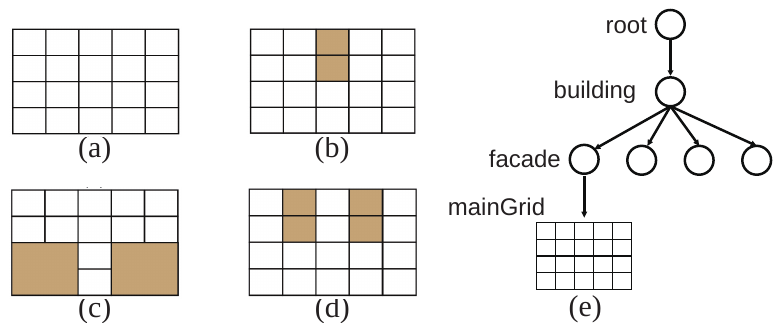
\includegraphics[width=13cm]{figuras/seletores.png}
	}
	{\Fonte{\cite{wonka2018}}}	
\end{figure}

\begin{figure}[h!]
	\centering
	\captionsetup{width=15cm}
	\Caption{\label{fig:agrupamento} Exemplo da utilização de funções de agrupamento.}
	\UFCfig{}{
		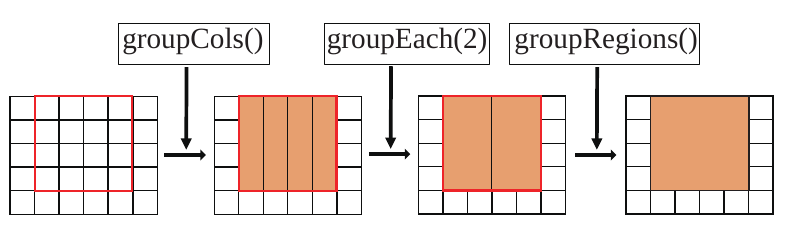
\includegraphics[width=13cm]{figuras/groups_selex.png}
	}
	{\Fonte{\cite{wonka2018}}}	
\end{figure}

\subsection{Ações}
\label{sec:selex_acoes}

As \textit{actions} são descritas por \citeonline{wonka2018} como funções que podem ser executadas sobre as formas retornadas por uma \textit{selection-expression}, sendo amplamente utilizadas para criar novas formas e as adicionar na hierarquia de formas, por exemplo, "\textit{addShape}", "\textit{attachShape}", "\textit{coverShape}" e "\textit{connectShape}". O pai de uma nova forma pode ser especificado explicitamente ou implicitamente utilizando valores padrões. Normalmente, o pai é a forma de construção de entrada ou, no caso de uma forma virtual, o primeiro ancestral que é uma forma de construção. A Figura \ref{fig:acoes_selex}(a) ilustra um exemplo da função "\textit{addShape}". Para gerar a fachada da Figura \ref{fig:cgaVSselex}, as instruções presentes na Figura \ref{fig:code_selex} fazem uso intensivo da função "\textit{addShape}", uma vez que o exemplo é 2D.

\citeonline{wonka2018} afirmam que outro aspecto da modelagem de edifícios residenciais complexos é a exigência de um controle cuidadoso da geometria que está sendo gerada. Para isto, são utilizados comandos para criar geometria dentro de formas que não são cobertas por outras formas com a função "\textit{coverShape}", conforme mostrado na Figura \ref{fig:acoes_selex}(b). Além disto, a \gls{SELEX} também fornece diversas funções para criar formas virtuais (grades), como no exemplo da Figura \ref{fig:acoes_selex}(c).

\begin{figure}[h!]
	\centering
	\captionsetup{width=15cm}
	\Caption{\label{fig:acoes_selex} Exemplo da utilização de \textit{actions}.}
	\UFCfig{}{
		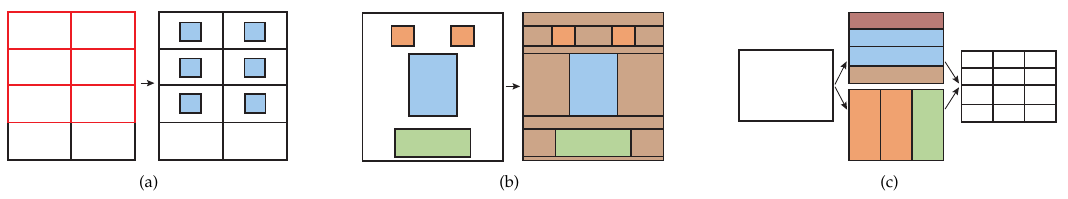
\includegraphics[width=15cm]{figuras/acoes_selex.png}
	}
	{\Fonte{\cite{wonka2018}}}	
\end{figure}

\subsection{Funções de restrição}
\label{sec:selex_funcoes}

Segundo \citeonline{wonka2018}, existe uma grande dificuldade para especificar a localização de uma forma em uma gramática estocástica, pois não é possível saber exatamente quais formas foram colocadas anteriormente e onde estão. Neste contexto, a \gls{SELEX} permite que seja definida uma sequência de restrições a partir do seguinte comando:

\vspace{0.3cm}

\begin{description}
    \item[] \qquad \qquad $constrain(constraint1, constraint2, ...)$.
\end{description}

\vspace{0.3cm}

\citeonline{wonka2018} consideram duas opções de \textit{design} para o problema de alinhamento. A primeira escolha de \textit{design} é decidir se as linhas de ajuste devem ser colocadas explicitamente por um comando, ou ser definidas implicitamente pelos limites das formas geradas numa etapa anterior. A segunda opção de \textit{design} é decidir se as linhas de ajuste devem ser nomeadas com um rótulo ou não. Na Figura \ref{fig:restricao_selex1}, é mostrado um exemplo comparando o ajuste com e sem rótulos, no qual: 

\begin{description}
    \item[] \; (a) Dado um \textit{layout} inicial com as formas $a$, $b$ e $c$;
    
    \item[] \; (b) Uma nova forma rotulada $d$ é adicionada;
    
    \item[] \; (c) No ajuste sem rótulos, a forma $d$ se encaixa nas linhas de ajuste mais próximas, ou seja, à esquerda da forma $a$ e à esquerda da forma $c$;
    
    \item[] \; (d) Utilizar ajuste com rótulos permite um controle mais preciso, por exemplo, ajustando a coordenada x ao centro da forma $d$ à coordenada x ao centro da forma $a$.
\end{description}

\begin{figure}[h!]
	\centering
	\captionsetup{width=15cm}
	\Caption{\label{fig:restricao_selex1} Comparação do ajuste com e sem o uso de rótulos.}
	\UFCfig{}{
		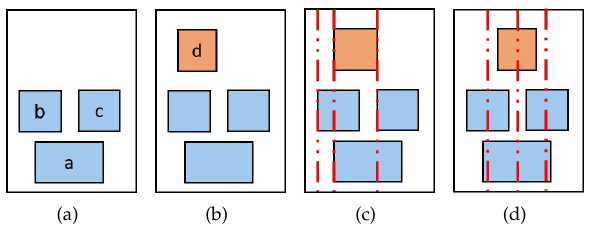
\includegraphics[width=15cm]{figuras/restricoes_selex1.png}
	}
	{\Fonte{\cite{wonka2018}}}	
\end{figure}

Conforme apresentado por \citeonline{wonka2018}, o alinhamento pode ser especificado de duas maneiras: uma forma de entrada ou uma forma de referência especificada por um rótulo. Os tipos de alinhamento suportados pela \gls{SELEX} são: "\textit{left}", "\textit{right}", "\textit{top}", "\textit{bottom}", "$center\mbox{-}x$", "$center\mbox{-}y$", "$one2two\mbox{-}x$" e "$one2two\mbox{-}y$". Por exemplo, a função:

\vspace{0.3cm}

\begin{description}
    \item[] \qquad \qquad \textit{constrain(snap2("window", "left"), snap2("window", "center\mbox{-}x"))}
\end{description}

\vspace{0.3cm}

\noindent especifica que uma forma de entrada deve ser alinhada à esquerda e ao centro x em relação a uma forma identificada como "\textit{window}". Os exemplos de "\textit{left}" \, e "$one2two\mbox{-}x$" \, são ilustrados na Figura \ref{fig:alinhamento_selex}, onde: (a) "\textit{left}" \, alinha a forma de entrada em verde a uma forma de referência em branco, e (b) "$one2two\mbox{-}x$" \, alinha a forma de entrada em verde ao centro da caixa delimitadora de duas formas de referência brancas. A linha tracejada vermelha indica a posição de ajuste, enquanto a caixa vermelha marca a delimitação de duas formas de referência.

\begin{figure}[h!]
	\centering
	\captionsetup{width=15cm}
	\Caption{\label{fig:alinhamento_selex} Dois exemplos de alinhamento.}
	\UFCfig{}{
		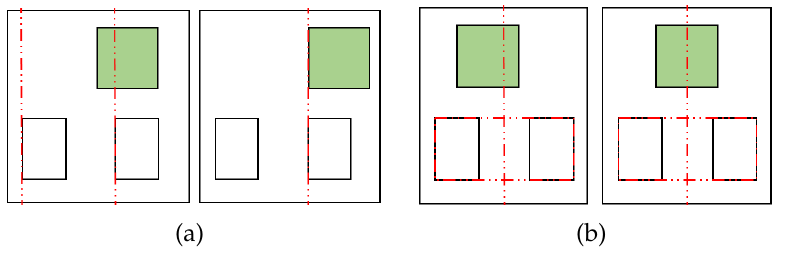
\includegraphics[width=13cm]{figuras/selex_alinhamento.png}
	}
	{\Fonte{\cite{wonka2018}}}	
\end{figure}

Especificações adicionais sobre a \gls{SELEX} foram disponibilizadas por \citeonline{wonka2018} como material suplementar.

\subsection{Comparativo}
\label{sec:comparativo}

Para evidenciar a simplicidade com que as regiões de uma fachada são representadas na árvore de formas, \citeonline{wonka2018} apresentam um exemplo ilustrativo, comparando o resultado da \textit{SELEX} com o resultado da \textit{CGA Shape}, conforme mostrado na Figura \ref{fig:arvore_cga_selex}(a) e Figura \ref{fig:arvore_cga_selex}(b), respectivamente. Neste caso, percebe-se que a árvore de formas produzida pela \textit{SELEX} apresenta uma estrutura mais plana, resultando em menos nós intermediários. Isto acontece pelo fato da \textit{SELEX} não possuir uma forma para representar os pisos, uma vez que o acesso das linhas e colunas pode ser facilmente realizado por meio de uma consulta na forma virtual.

\begin{figure}[h!]
	\centering
	\captionsetup{width=15cm}
	\Caption{\label{fig:arvore_cga_selex} Exemplo da árvore de formas gerada pela \textit{CGA Shape} em (a), e pela \textit{SELEX} em (b), com base na fachada (c).}
	\UFCfig{}{
		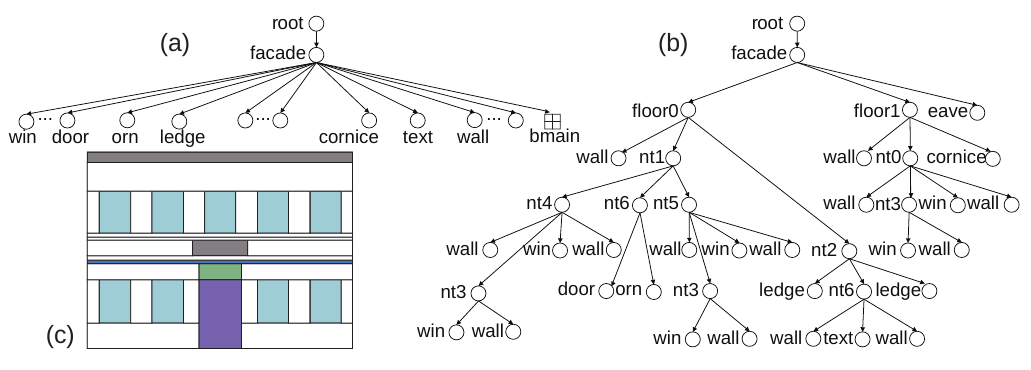
\includegraphics[width=15cm]{figuras/arvore_cga_selex.png}
	}
	{\Fonte{\cite{wonka2018}}}	
\end{figure}

\newpage

Ainda abordando estas duas técnicas, \citeonline{wonka2018} apresentam outros três exemplos, mostrados na Figura \ref{fig:estatisticas_selex_cga}, fazendo um comparativo entre a quantidade de regras \textit{r} para gerar as fachadas; o número de operações \textit{o}; o número de linhas \textit{l}; o número de palavras \textit{w}; e o número de caracteres \textit{c}. Neste caso, os dados referentes à \textit{CGA Shape} estão entre parênteses.

\begin{figure}[h!]
	\centering
	\captionsetup{width=15cm}
	\Caption{\label{fig:estatisticas_selex_cga} Estatísticas da \textit{SELEX} e \textit{CGA Shape} para geração de fachadas.}
	\UFCfig{}{
		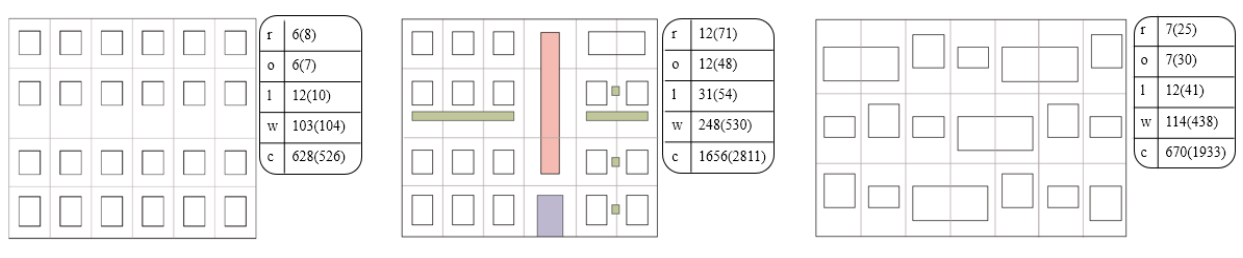
\includegraphics[width=16cm]{figuras/comp_selex_cga.png}
	}
	{\Fonte{\cite{wonka2018}}}	
\end{figure}

\subsection{Aplicações}
\label{sec:selex_modelagem}

Nas Figuras \ref{fig:exemplo_selex} e \ref{fig:exemplo_selex_arvore}, \citeonline{wonka2018} ilustram a utilização de formas virtuais e \textit{selection-expressions} no processo de modelagem de um edifício, a partir das seguintes etapas:

\begin{description}
    \item[] \; (a) Polígono da planta especificada pelo usuário;
    
    \item[] \; (b) Uma operação de extrusão é aplicada ao polígono da planta, gerando um edifício;
    
    \item[] \; (c) Todas as fachadas do edifício são divididas em andares, por meio da inclusão de uma grade como forma virtual;
    
    \item[] \; (d) Cada fachada herda as informações do piso e é dividida em uma grade mais fina, especificando colunas, que são rotuladas com "\textit{colLeft}", "\textit{colMidLeft}", "\textit{colMidRight}" \, e "\textit{colRight}";
    
    \item[] \; (e) As colunas são selecionadas pelo rótulo "\textit{colMidLeft}";
    
    \item[] \; (f) As colunas são selecionadas pelo rótulo "\textit{colMidRight}" \, e a operação \textit{push} é aplicada na região rotulada com "\textit{colMidLeft}";
    
    \item[] \; (g) As colunas são selecionadas pelo rótulo "\textit{rowDown}" \,e a operação de \textit{pull} é aplicada nas regiões rotuladas com "\textit{colMidRight}" \, e "\textit{rowDown}", formando a massa do edifício;
    
    \item[] \; (h) Uma sub-região no lado esquerdo é selecionada e uma sub-grade é adicionada;
    
    \item[] \; (i) Conjuntos de células na grade principal são selecionadas para adicionar formas abrangendo várias células;
    
    \item[] \; (j) Linhas pares/ímpares em uma sub-região da segunda linha à última linha são selecionadas;
    
    \item[] \, (k) Uma forma de conexão é selecionada;
    
    \item[] \; (l) Linhas pares/ímpares são selecionadas e sub-grades diferentes são adicionadas;
    
    \item[] (m) Colunas largas e estreitas são selecionadas para adicionar janelas;
    
    \item[] \, (n) Janelas e portas extras são adicionadas;
    
    \item[] \, (o) Complementos são adicionados.
\end{description}

\begin{figure}[h!]
	\centering
	\captionsetup{width=15cm}
	\Caption{\label{fig:exemplo_selex} Exemplo de modelagem utilizando \gls{SELEX}.}
	\UFCfig{}{
		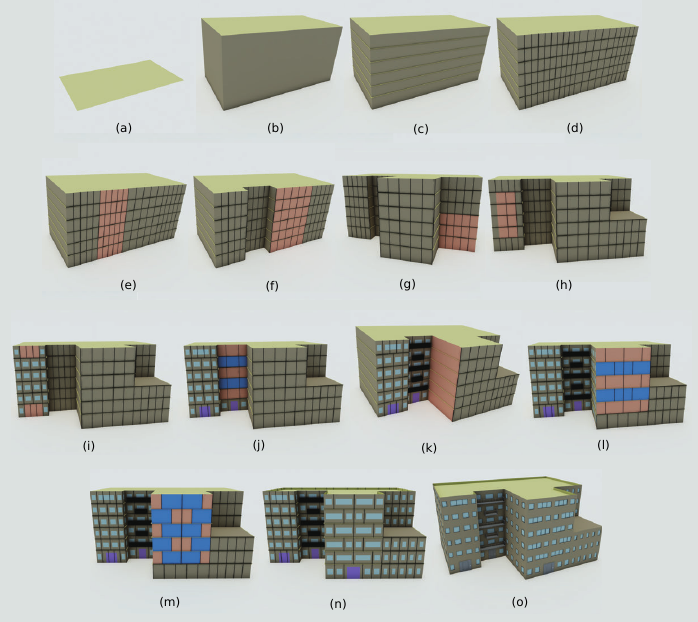
\includegraphics[width=15cm]{figuras/selex_exemplo_001.png}
	}
	{\Fonte{Adaptado de \cite{wonka2018}}}	
\end{figure}

\begin{figure}[h!]
	\centering
	\captionsetup{width=15cm}
	\Caption{\label{fig:exemplo_selex_arvore} Árvore de formas construída com base no modelo final da Figura \ref{fig:exemplo_selex}(o).}
	\UFCfig{}{
		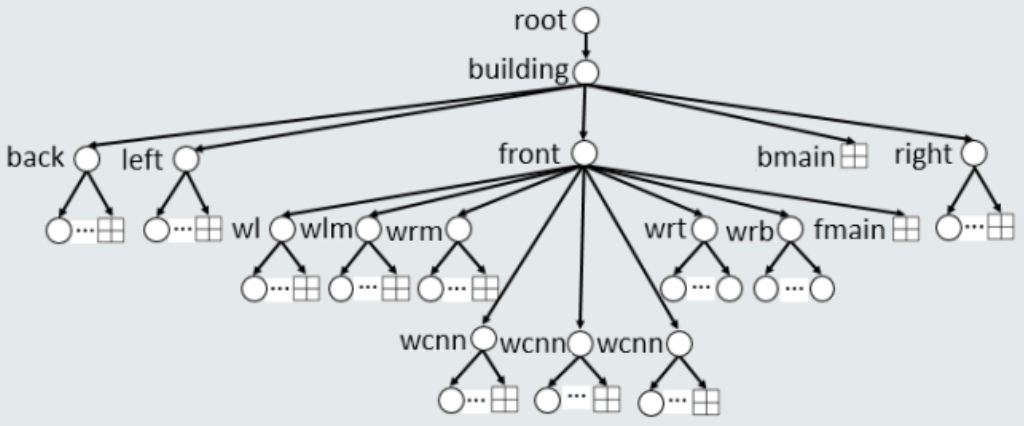
\includegraphics[width=15cm]{figuras/arvore_final.png}
	}
	{\Fonte{Adaptado de \cite{wonka2018}}}	
\end{figure}

\vspace{1cm}

Por fim, após a apresentação das especificações, dos exemplos ilustrativos, e da análise do desempenho da \textit{SELEX} em relação às suas precursoras, pode-se perceber que tal técnica representa um grande avanço no campo da modelagem procedural de edifícios. Assim, na próxima seção, será abordado o conceito de deformação, bem como sua relação com a modelagem procedural.

\newpage

\section{Deformação}
\label{sec:deformacao}

No campo da Física, a deformação de uma estrutura é qualquer mudança da configuração geométrica do corpo que leve a uma variação da sua forma ou das suas dimensões, após a aplicação de uma ação externa \cite{truesdell1992}. Na área da Computação Gráfica, por sua vez, a modelagem de sólidos é uma das técnicas essenciais utilizadas em modeladores 3D comuns, como Maya, Rhinoceros e Blender, onde a modificação dos objetos é realizada, frequentemente, por meio da deformação de forma livre \cite{jana2017}.

%Baseado neste contexto, a próxima seção é voltada para uma breve apresentação de algumas técnicas de deformação existentes. 

% Pois não existe outra subseção
%\subsection{Técnicas de deformação}
%\label{sec:tecnicas_deformacao}

Idealizada por \citeonline{sedeberg1986}, a deformação de forma livre é uma transformação do espaço. Nela, é definida uma grade regular de pontos de controle, os quais podem ser descritos por uma combinação linear. Ao deslocar estes pontos de controle, uma deformação do espaço é alcançada. Geralmente, estes pontos de controle são espaçados regularmente na caixa delimitadora do elemento a ser deformado, conforme ilustrado na Figura \ref{fig:sedeberg}.

\begin{figure}[h!]
	\centering
	\captionsetup{width=15cm}
	\Caption{\label{fig:sedeberg} À esquerda, um exemplo de deformação livre dos objetos do cenário, a partir da mudança dos pontos da grade cúbica visível à direita.}
	\UFCfig{}{
		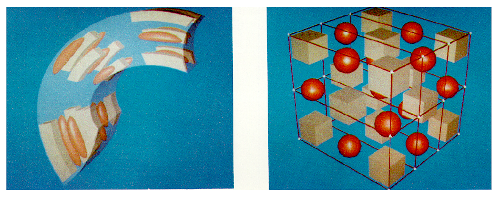
\includegraphics[width=13cm]{figuras/sedeberg.png}
	}
	{\Fonte{\cite{sedeberg1986}}}	
\end{figure}

Uma evolução do trabalho de \citeonline{sedeberg1986} é trazida por \citeonline{jin2000}, onde é apresentado um método de deformação tridimensional utilizando coordenadas polares direcionais. O usuário especifica um objeto de controle de origem e um objeto de controle de destino (Figura \ref{fig:jin_exemplo1}), que atuam como espaços de incorporação. Os objetos de controle de origem e de destino determinam uma transformação de volume tridimensional, que mapeia o espaço anexado no objeto de controle de origem para o espaço do objeto de controle de destino (Figura \ref{fig:jin_exemplo2}). Ao incorporar o objeto a ser deformado no objeto de controle de origem, a transformação ocorre sem o movimento dos pontos de controle.

\begin{figure}[h!]
	\centering
	\captionsetup{width=15cm}
	\Caption{\label{fig:jin_exemplo1} Objeto de controle de origem (a) e objetos de destino (b), (c), (d). Neste caso, $O_S$ e $O_D$ representam os respectivos centros dos objetos.}
	\UFCfig{}{
		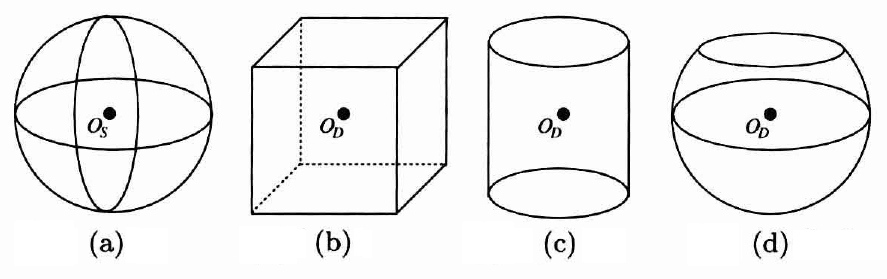
\includegraphics[width=12cm]{figuras/jin_exemplo1.png}
	}
	{\Fonte{Adaptado de \cite{jin2000}}}	
\end{figure}

\begin{figure}[h!]
	\centering
	\captionsetup{width=15cm}
	\Caption{\label{fig:jin_exemplo2} Deformação de uma bola de futebol (a) com base nos objetos (b), (c) e (d), da Figura \ref{fig:jin_exemplo1}.}
	\UFCfig{}{
		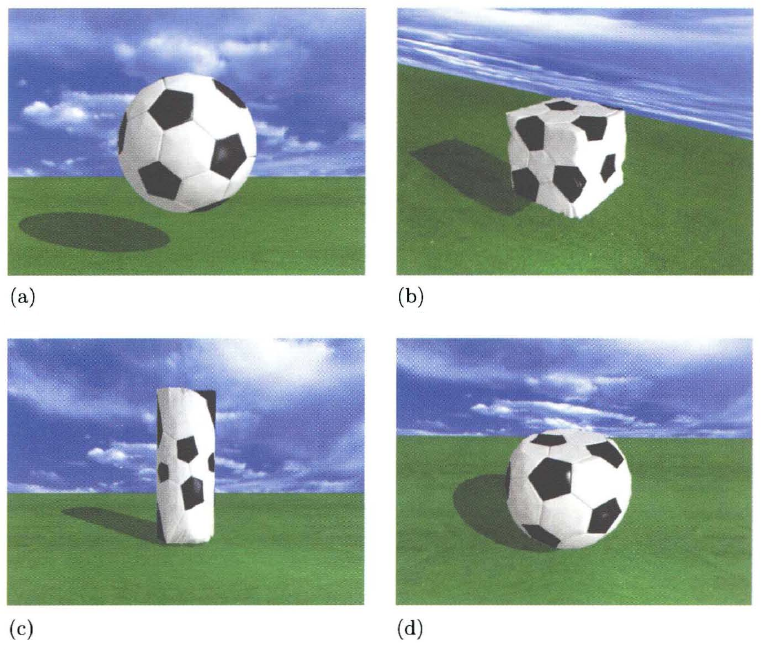
\includegraphics[width=10cm]{figuras/jin_exemplo2.png}
	}
	{\Fonte{Adaptado de \cite{jin2000}}}	
\end{figure}

Outras duas técnicas são apresentadas por \citeonline{jana2017}, o esquema de \citeonline{sedeberg1986} baseado em polinômios de Bernstein, que é a base das técnicas de deformação de forma livre (Figura \ref{fig:sedeberg_ffd}), e o método \gls{NURBS}, que utiliza um escopo mais elaborado e operações mais complexas (Figura \ref{fig:nurbs_ffd}).

\begin{figure}[h!]
	\centering
	\captionsetup{width=15cm}
	\Caption{\label{fig:sedeberg_ffd} Técnica de deformação de forma livre de Sederberg: a) antes e b) depois da transformação.}
	\UFCfig{}{
		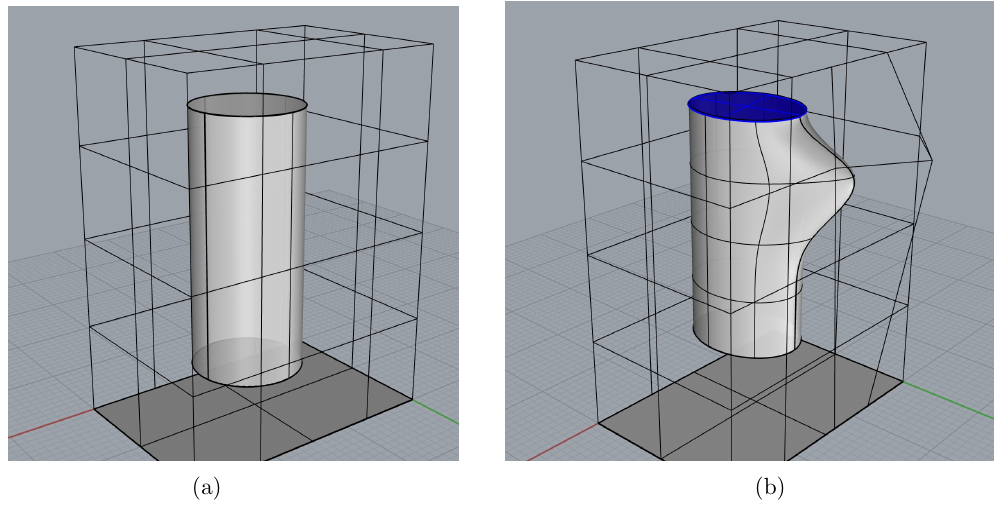
\includegraphics[width=12cm]{figuras/sedeberg_ffd.png}
	}
	{\Fonte{\cite{jana2017}}}	
\end{figure}

\begin{figure}[h!]
	\centering
	\captionsetup{width=15cm}
	\Caption{\label{fig:nurbs_ffd} Técnica de deformação de forma livre utilizando \gls{NURBS}: a) antes e b) depois da transformação.}
	\UFCfig{}{
		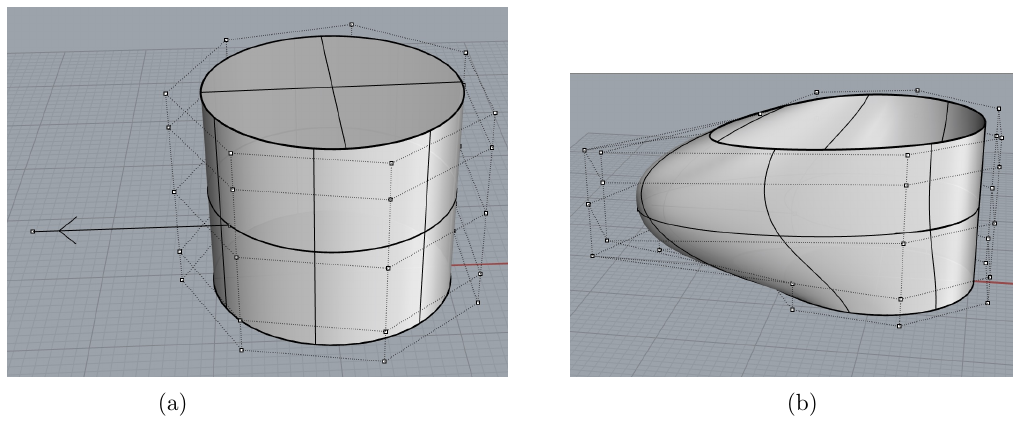
\includegraphics[width=12cm]{figuras/nurbs_ffd.png}
	}
	{\Fonte{\cite{jana2017}}}	
\end{figure}

Por achar o uso de caixas insatisfatório, \citeonline{fellner2013} argumentam que uma maior variedade de formas pode ser obtida pelo uso de poliedros convexos como delimitador de volumes, pois as operações de divisão não ficam mais limitadas aos três eixos principais, podendo-se utilizar planos arbitrários. Um exemplo é mostrado na Figura \ref{fig:convex_example}, onde: (a) em um poliedro convexo, (b) um orifício circular é cortado deixando dois resultados, (c) uma parte interna convexa e (d) os arredores não convexos. A borda vermelha mostra o escopo convexo correspondente, que é igual ao escopo original.

\begin{figure}[h!]
	\centering
	\captionsetup{width=15cm}
	\Caption{\label{fig:convex_example} Operação de deformação introduzida por \citeonline{fellner2013}.}
	\UFCfig{}{
		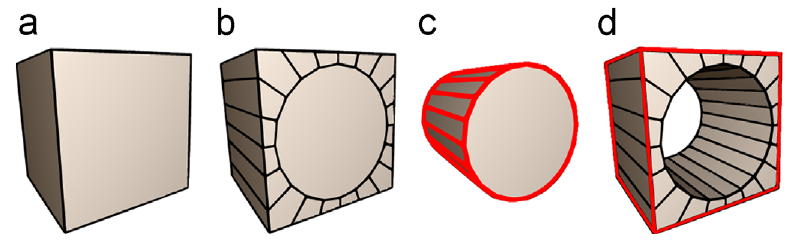
\includegraphics[width=11cm]{figuras/convex_polyhedra.png}
	}
	{\Fonte{\cite{fellner2013}}}	
\end{figure}

As \textit{deformation grammars}, por sua vez, foram introduzidas por \citeonline{vimont2017}, permitindo deformar livremente objetos complexos ou conjuntos de objetos, preservando sua consistência. Esta abordagem processa deformações de objetos como símbolos, através das regras de interpretação definidas pelo usuário. Um exemplo é mostrado na Figura \ref{fig:vimont}.

\begin{figure}[h!]
	\centering
	\captionsetup{width=15cm}
	\Caption{\label{fig:vimont} O modelo inicial de uma casa (a) é deformado pelo usuário, enquanto preserva as propriedades típicas, como a ortogonalidade da parede e a disposição linear do piso (b).}
	\UFCfig{}{
		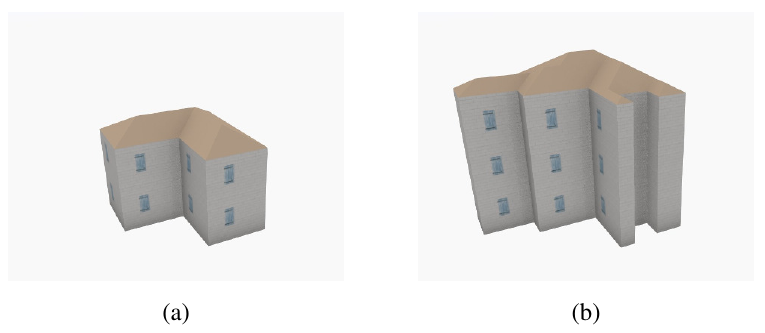
\includegraphics[width=13cm]{figuras/deformation_grammar.png}
	}
	{\Fonte{\cite{vimont2017}}}	
\end{figure}

\vspace{1cm}

Neste capítulo, foram apresentadas algumas das principais técnicas que surgiram no decorrer da história para geração procedural de edifícios, abordando suas características, alguns exemplos de aplicação, e também suas limitações. Por meio de uma análise comparativa, percebeu-se que o emprego de \textit{Selection Expressions}, a mais recente das abordagens, apresenta diversas vantagens em relação às suas precursoras, \textit{CGA Shape} e \textit{CGA++}. Contudo, mesmo com a introdução de tais melhorias pela \gls{SELEX}, ainda existem modelos que estão além da sua capacidade de modelagem, como é o caso de edifícios com arquitetura arredondada. Assim, visando contextualizar este cenário, no próximo capítulo, serão abordadas algumas técnicas voltadas para a resolução de questões similares.
